\documentclass[12pt]{"article"}
\setlength{\parindent}{0pt}
\linespread{1.5}
\usepackage[margin=1.5in]{geometry}
\usepackage{graphicx}
\graphicspath{ {../Figures/} }
\usepackage{titlesec}
\newcommand{\sectionbreak}{\clearpage}
\usepackage{sidecap}
\usepackage[singlelinecheck=false, labelfont=bf]{caption}
\usepackage{verbatim}
\usepackage{setspace}
\newcommand{\mycaption}[2]{\caption[#1]{\textbf{#1.} #2}}
\usepackage{chngcntr}
\counterwithin{figure}{section}


\begin{document}

\begin{titlepage}
\centering
{\huge Title\\}
\end{titlepage}


\pagebreak

\begin{Large}
\textbf{Abstract}\\
\end{Large}


\pagebreak

\begin{Large}
\textbf{Impact statement}\\
\end{Large}


\pagebreak

\begin{Large}
\textbf{Acknowledgements}\\
\end{Large}


\tableofcontents
\listoffigures


%%%%%%%%%%%%%%%%%%%%%%%%%%%%%%%%%%%%%%%%%%%%%%%%%%%%%%%%%%
\clearpage
\section{Introduction}

\subsection{Spatial patterning in biological systems}

\clearpage
\subsection{Cell polarity}

\clearpage
\subsection{Maintenance of cell polarity by bistable reaction-diffusion systems}
\subsubsection{Bistable reaction kinetics}
\subsubsection{Single species polarity models}
\subsubsection{The mutual antagonism model}

\clearpage
\subsection{A molecular basis for ultrasensitivity}
\subsubsection{Ultrasensitivity in protein phosphorylation reactions}
\subsubsection{Ultrasensitivity through cooperative membrane binding}

\clearpage
\subsection{PAR polarity in C elegans zygotes}
\subsubsection{Mechanisms of PAR cortical association}
\subsubsection{Maintenance of polarity by mutual antagonism}
\subsubsection{Establishment of polarity}
\subsubsection{Downstream of the PAR proteins}
\subsubsection{Resistance and substrate competition}
\subsubsection{Discussion}

\clearpage
\subsection{PAR-2: roles and mechanisms of action}
\subsubsection{Main functional roles of PAR-2}
\subsubsection{Evidence and proposed roles for oligomerisation}
\subsubsection{Roles for the RING domain}

\clearpage
\subsection{RING domains across the proteome}
\subsubsection{RING proteins in the ubiquitination pathway}
\subsubsection{RINGs as dimerisation domains}
\subsubsection{Discussion}

%%%%%%%%%%%%%%%%%%%%%%%%%%%%%%%%%%%%%%%%%%%%%%%%%%%%%%%%%%
\clearpage
\section{A pipeline for quantification of membrane and cytoplasmic protein concentrations}

Text

\subsection{Autofluorescence correction}

Note: this section has been adapted from (Rodrigues, Bland), and describes work performed in conjunction with Nelio Rodrigues.

\subsubsection{Autofluorescence in C elegans}

One major barrier in quantitative experiments using C elegans is autofluorescence. Whilst usually minor in red channels excited with xxx wavelengths, autofluorescence is particularly prominent in channels excited with blue wavelengths which are commonly used to image green fluorophores. When using endogenously tagged proteins, which are often expressed at low levels, this contribution is often be a significant fraction of the total signal, and can therefore significantly obscure the true signal that one is interested in. This might pose particular problems for quantitative experiments, where the absolute signal levels may be important.\\

We can observe this problem by imaging untagged control embryos. As shown in (fig x), a significant amount signal is collected in the GFP channel, which varies both spatially within the image, and between different images. By comparison, total signal in embryos endogenously tagged with LGL GFP is also highly variable, and only marginally higher than N2s, suggesting that a significant fraction of the total signal observed in these cells is autofluorescence, and that the intra-embryo signal variation is largely due to variable autofluorescence. Despite being enriched on the posterior cortex, which is easily visible in cells with overexpressed LGL (ref), this is difficult to visualise here as a result of autofluorescence. Therefore, if we want to accurately visualise, and indeed quantify, protein levels and distributions, we need a method that can locally correct AF on a pixel-by-pixel basis.\\

% figure demonstrating autofluorescence

One approach that has been used for this is spectral imaging. Typically used to separate overlapping fluorophore signals based on spectral characteristics, this approach can also be used to separate out autofluorescence by treating it much like a fluorophore with its own spectral characteristics. Whilst often effective, these techniques require specialised instruments and analysis tools and cannot be performed on standard confocal microscopes.\\

However, simpler approaches have been used. By exploiting the fact that autofluorescence can often be described as a single component, with an emission spectrum much broader than GFP, one can find an emission wavelength (usually red) that is specific for autofluorescence, and use this channel to infer the amount of autofluorescence in the sample. This can then be subtracted away from the fluorophore channel, giving a ‘clean’ readout of fluorophore signal. In comparison to full spectral imaging, this method can be carried out with standard light sources and emission filters, and therefore can be easily implemented into existing workflows.\\

Inspired by this work, we aimed to implement, and assess the applicability of such a method to images of C elegans zygotes. In doing so, we have put together a robust and easily-implementable workflow which we’ve termed SAIBR: Spectral Autofluorescence Image correction by regression.\\


\subsubsection{SAIBR: a simplified method for autofluorescence correction based on dual emission imaging}


At minimum, autofluorescence correction relies on the ability to find a reporter channel that is free of GFP signal, but rich in autofluorescence, such that this channel can be used an independent readout of autofluorescence in the sample. Full spectral analysis performed by Nelio Rodrigues (not shown here), shows that red shifted emission filters, which are commonly used to image red fluorescent proteins, meet such a requirement.\\

Furthermore, by imaging untagged embryos with both the standard GFP channel and the AF channel, we find a strong linear correlation between pixel data from the two channels. Whilst raw pixel values do not correlate well, as these are dominated by noise, we can get a strong correlation by first applying a Gaussian filter to suppress this noise (fig x). We found that this relationship is consistent between embryos (fig x b, c). Furthermore, we found a near identical relationship when plotting the mean intensity values of individual embryos, suggesting that the same relationship can account for both intra- and inter-embryo AF variation. \\

\begin{figure}[!h]
\includegraphics[scale=0.95]{saibr_n2_correlation}
\setlength{\abovecaptionskip}{20pt}
\centering
\mycaption{Title}{Caption}
\end{figure}


Together, this implies that taking an autofluorescence channel image is sufficient to accurately predict the level of autofluorescence in the GFP channel. To quantify the necessary inter-channel conversion factor, I performed linear regression, using an ordinary least squares method, on Gaussian-filtered pixel values pooled from multiple untagged embryos. Then, to perform correction on images containing fluorophore, we just need to capture an autofluorescence channel image, alongside the GFP channel image, rescale the image according to this predefined relationship, and then subtract this away from the GFP channel image.\\


\clearpage
\subsubsection{Assessing performance on images of PAR proteins}

To assess the effectiveness of SAIBR, and it’s utility in the analysis of PAR proteins, I applied it to a range of images of unlabelled and GFP-labelled embryos. As expected, applying SAIBR to images of unlabelled cells reduced fluorescence from across the cell to zero, with no visible structures remaining. This is a good validation of the method, and suggests that it can properly account for all of the autofluorescence in the cell. \\

As already shown, images of LGL are dominated by autofluorescence, and so SAIBR was expected to be particularly useful. As shown in fig x, SAIBR strongly reduces signal within the cell, and improves contrast at the posterior cortex, allowing us to better resolve cortical enrichment at the posterior. Improvements are similar for PAR-3. In addition to improvements at the cortex, we see that SAIBR can suppress the local fluorescence minimum at the cell centre caused by lower AF at the pronuclei. For PAR-6 the improvements are qualitatively less striking, due to a higher ratio of fluorophore signal to autofluorescence, but nonetheless quantitatively important.\\

\begin{figure}[!h]
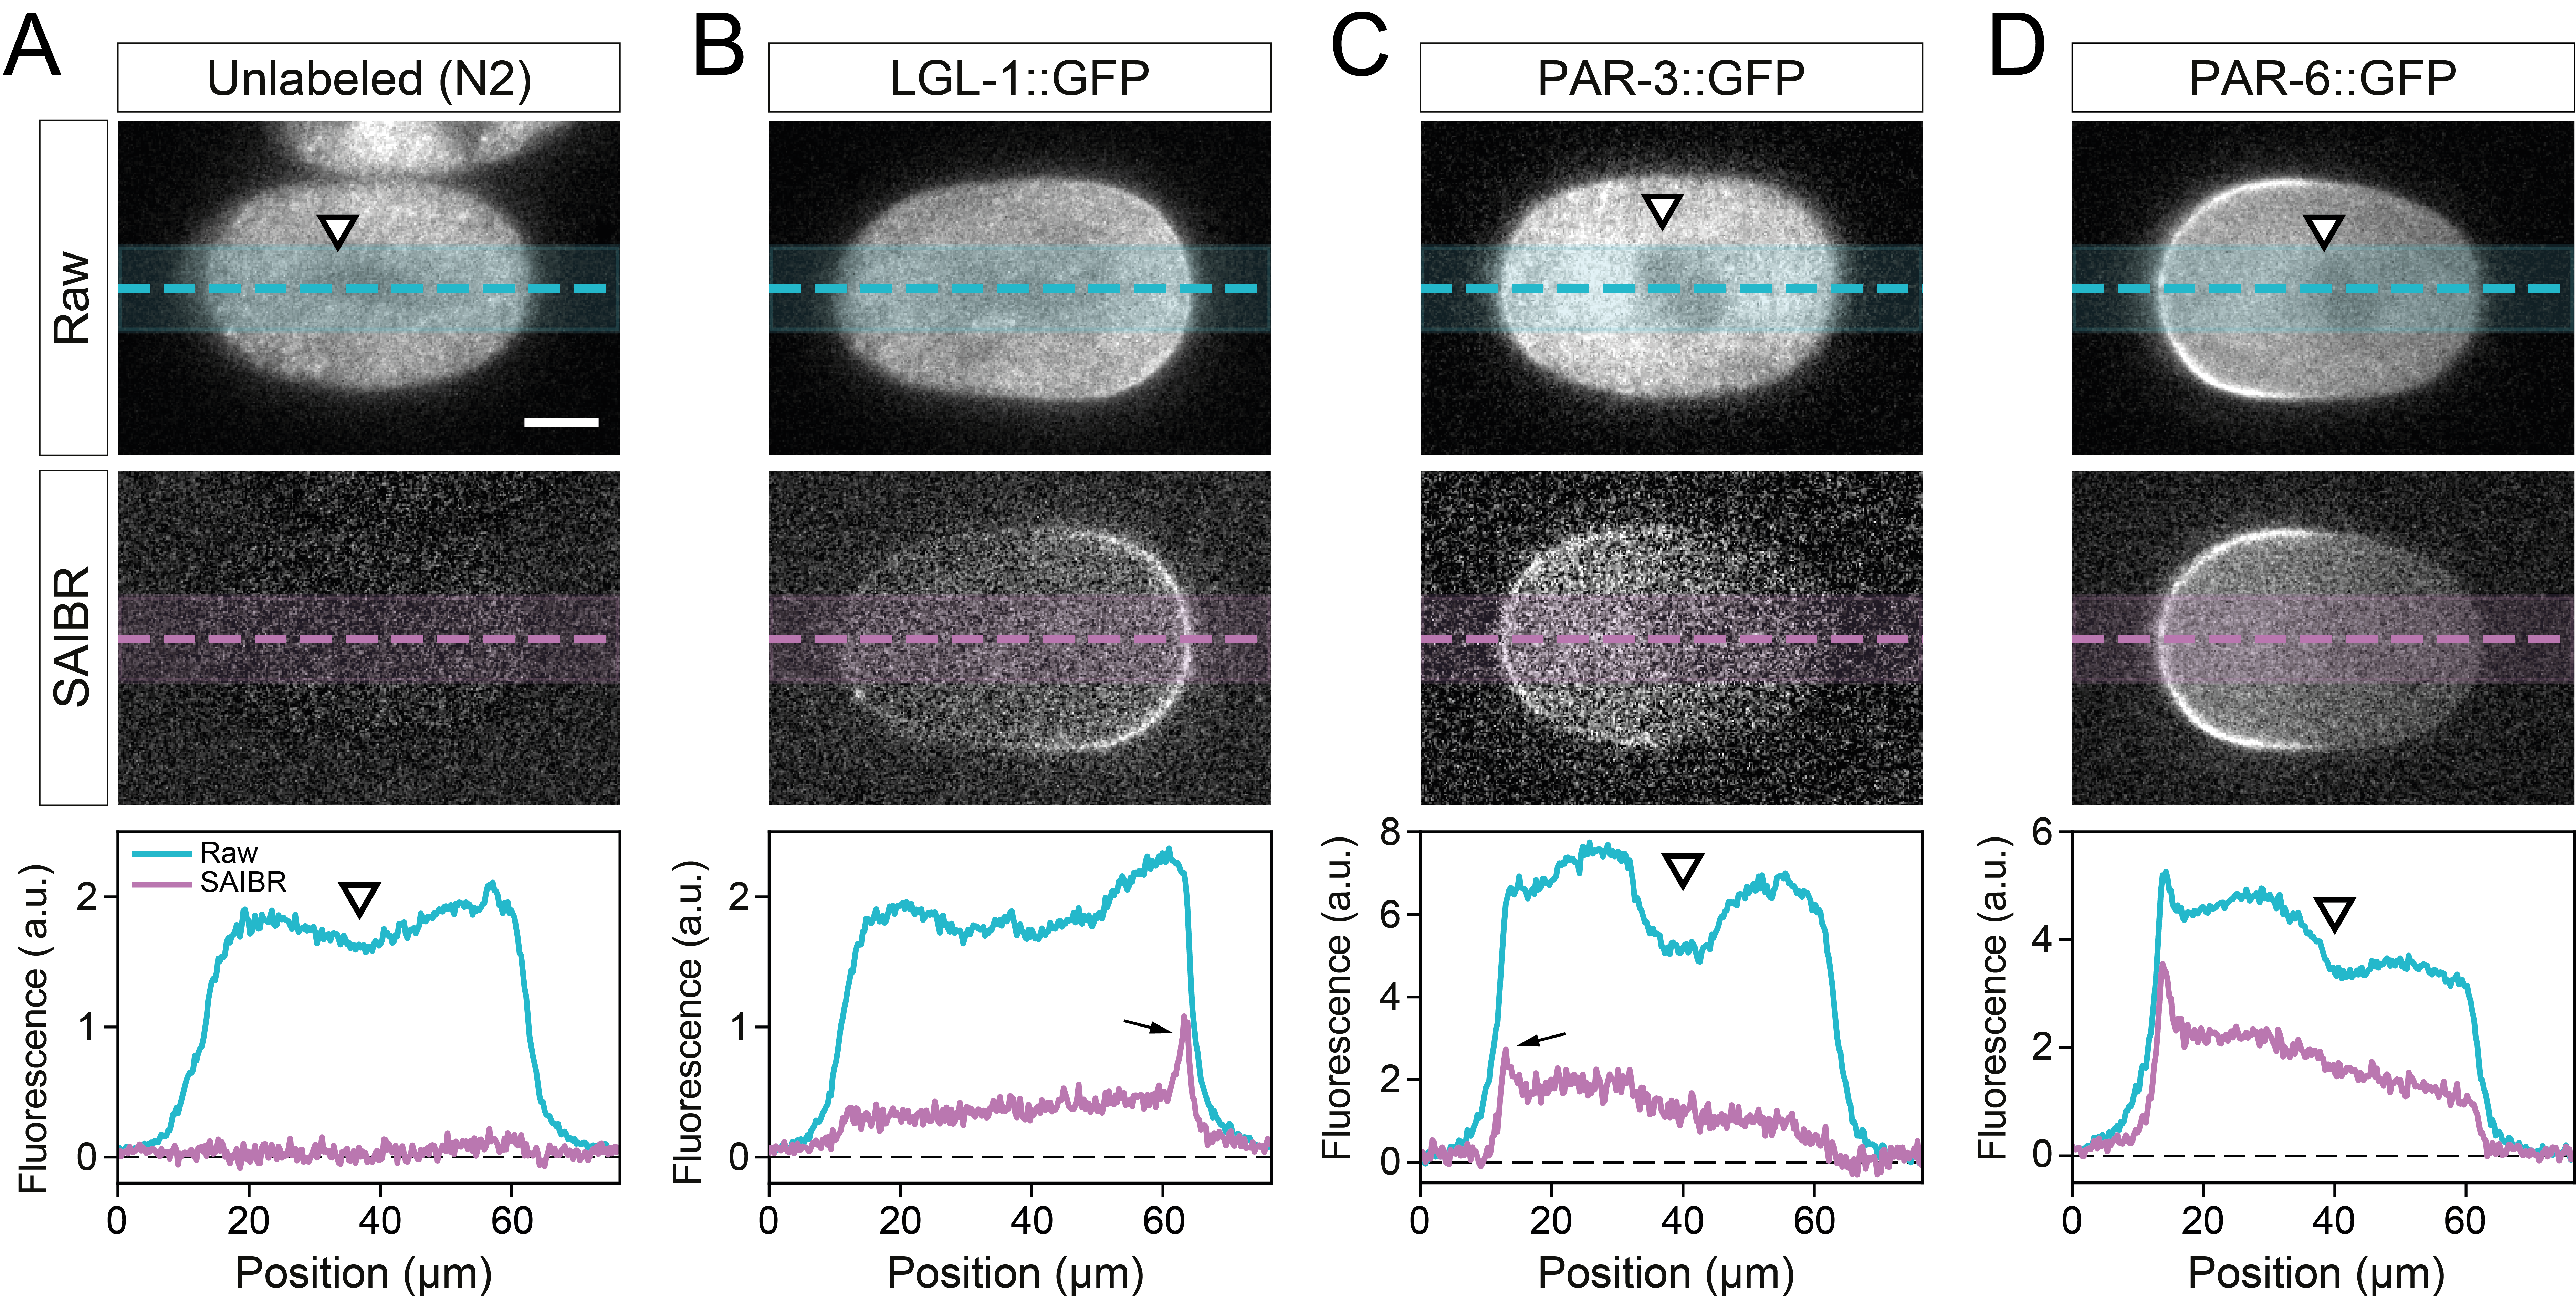
\includegraphics[scale=0.9]{saibr_spatial_correction}
\setlength{\abovecaptionskip}{20pt}
\centering
\mycaption{Title}{Caption}
\end{figure}

As shown in fig x, SAIBR has a strong impact on the shape of intensity profiles taken across the cortex within each polarity domain, in all cases showing a clearer peak and suppression of signal at the internal portion of the curves. As discussed in the next section, this has a particular importance for quantification of membrane and cytoplasmic concentrations.\\

\begin{figure}[!h]
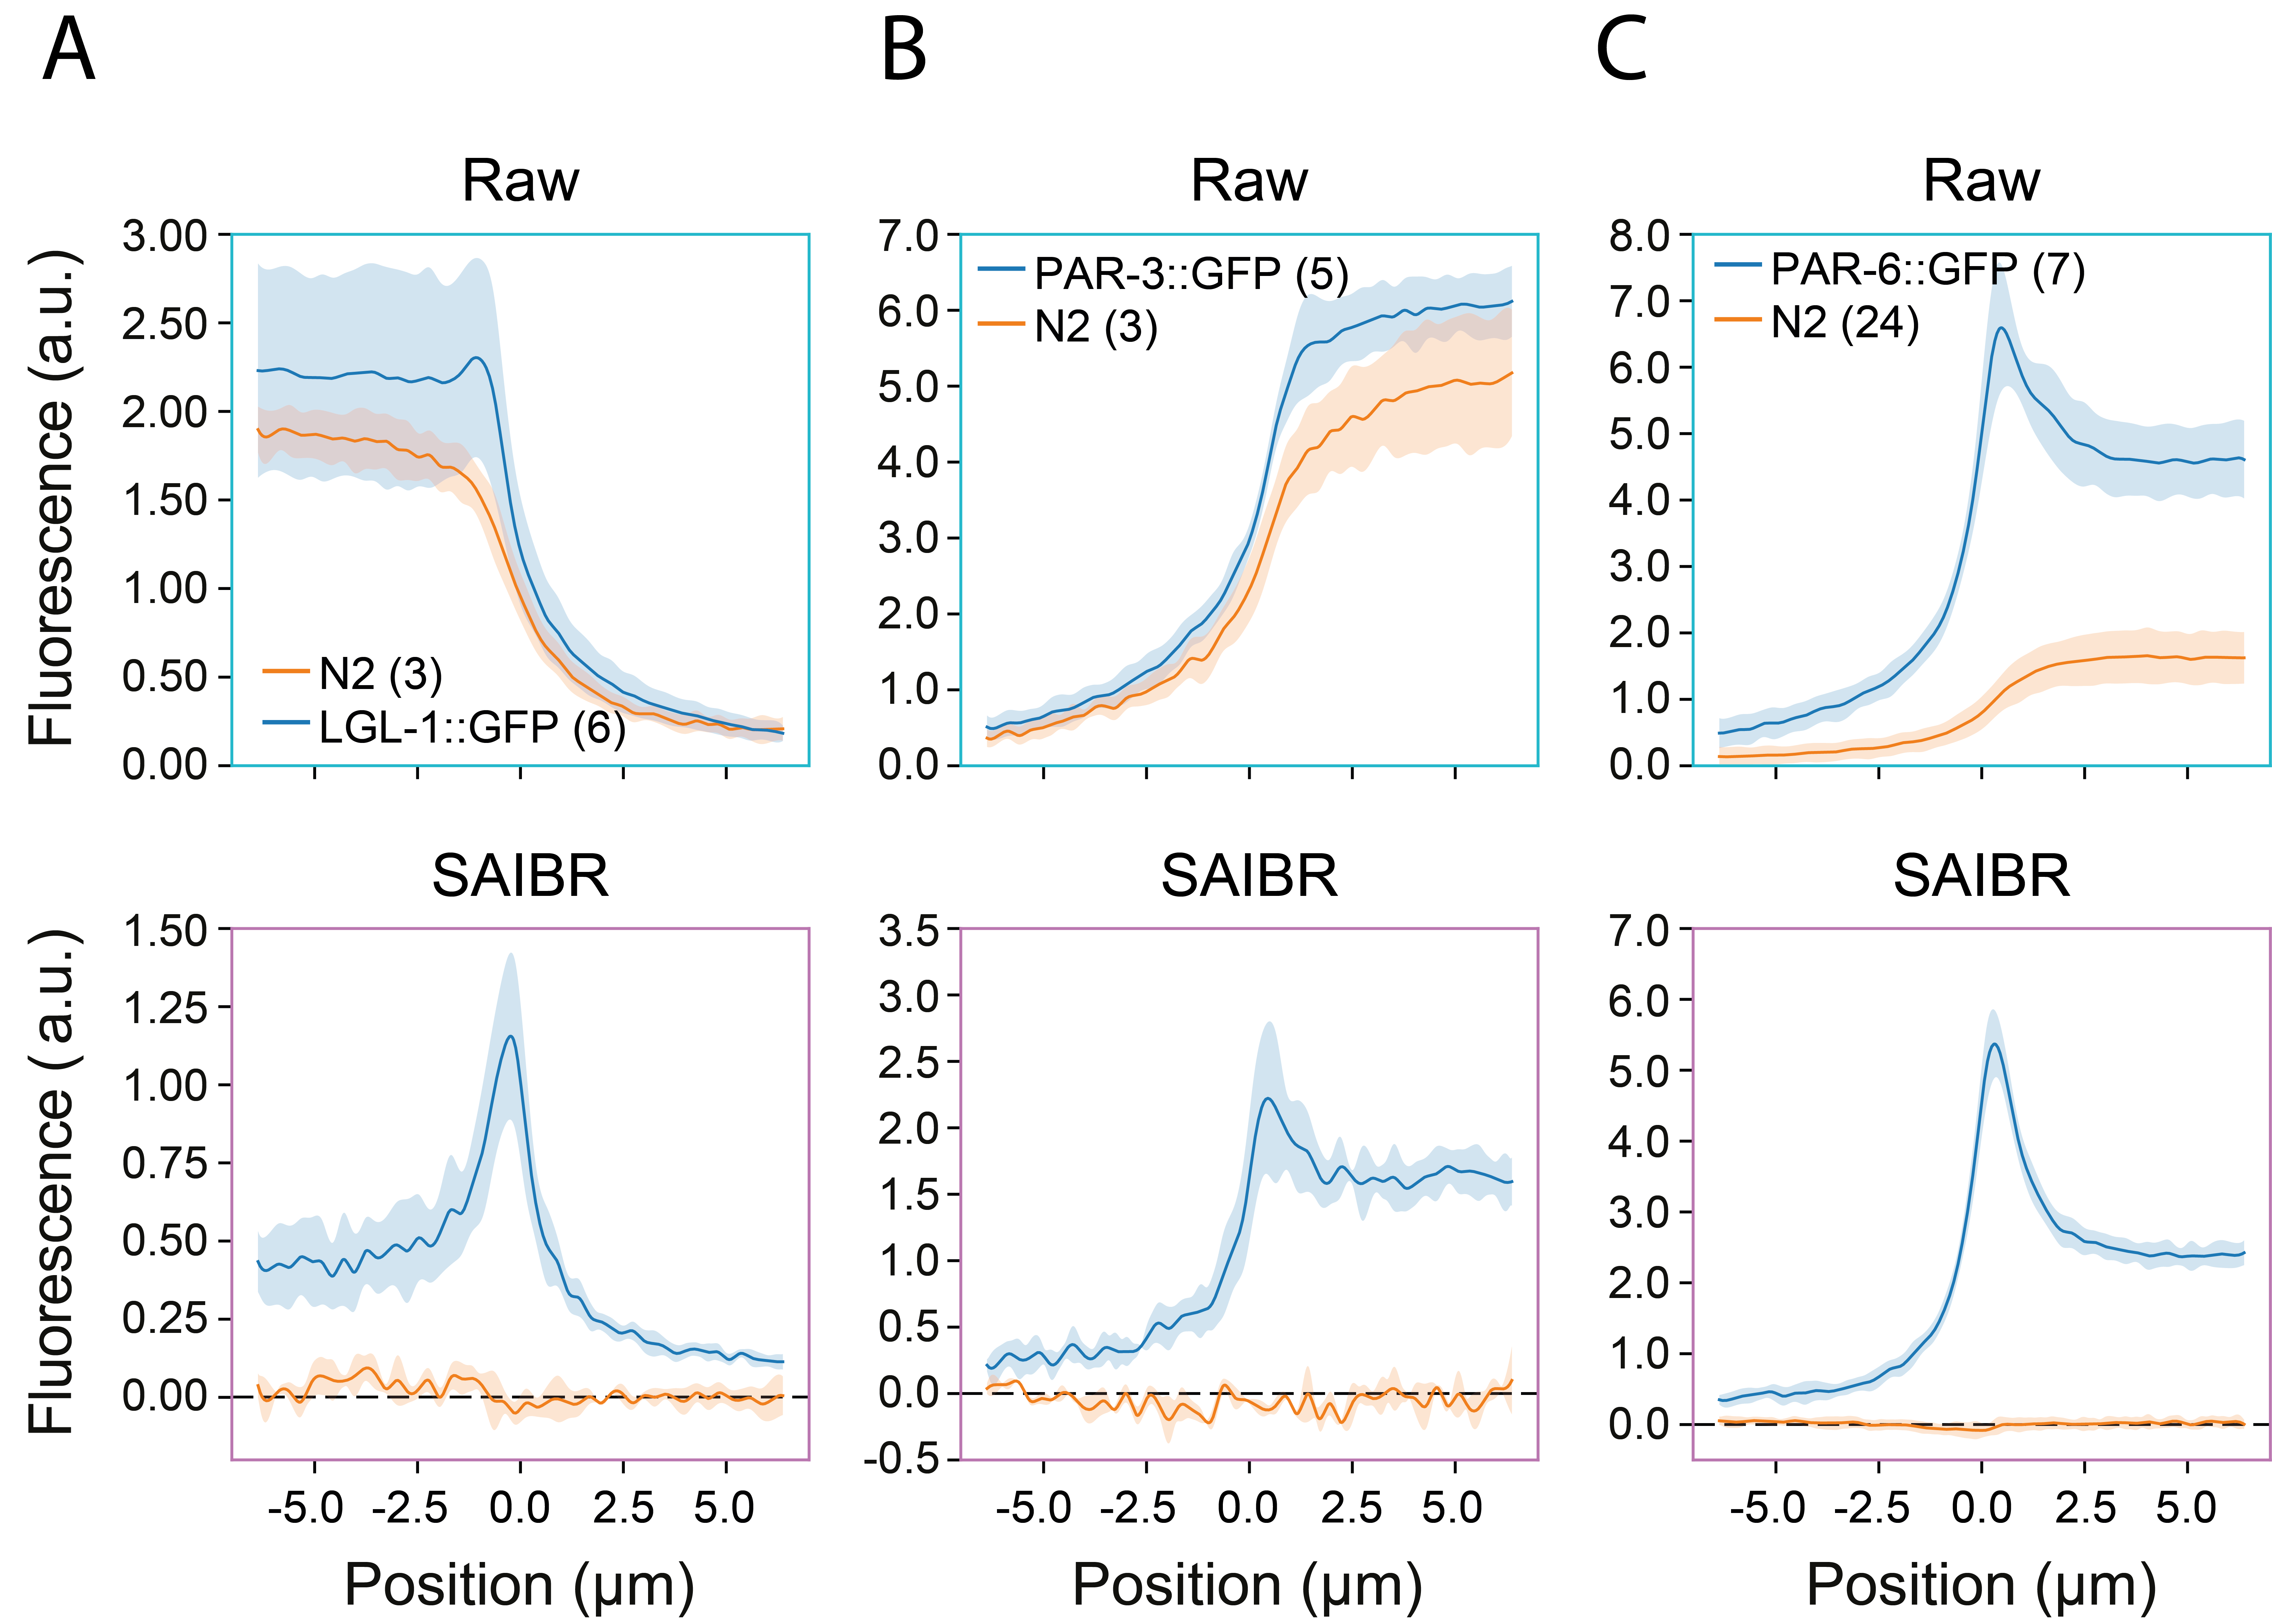
\includegraphics[scale=1]{saibr_membrane_profiles}
\setlength{\abovecaptionskip}{20pt}
\centering
\mycaption{Title}{Caption}
\end{figure}

\clearpage
\subsubsection{Extending SAIBR to dual-labelled C elegans embryos}

As SAIBR relies on a red shifted emission channel, complications can arise when there is a red fluorophore present. As red fluorophores are usually weakly excited by blue lasers, they will contribute additional signal to the AF channel, which may lead to overestimation, and therefore oversubtraction, of autofluorescence if not accounted for. If RFP levels are low, this effect may be small and can be ignored. However, if RFP levels are high, this bleedthrough effect can be significant. This can be demonstrated by observing the inter-channel relationship in control embryos tagged with a red fluorophore (fig x). We find that, when an RFP is present, this relationship deviates significantly from the typical relationship observed in N2s, in direct proportion to local RFP levels (fig x inset). As this relationship is linear, autofluorescence in the GFP channel can now be described as a linear function of both the AF and the RFP channels. Plotting the pixel data in three dimensions shows that the data can be successfully fit to a plane, by performing multiple linear regression (fig x). \\


\begin{figure}[!h]
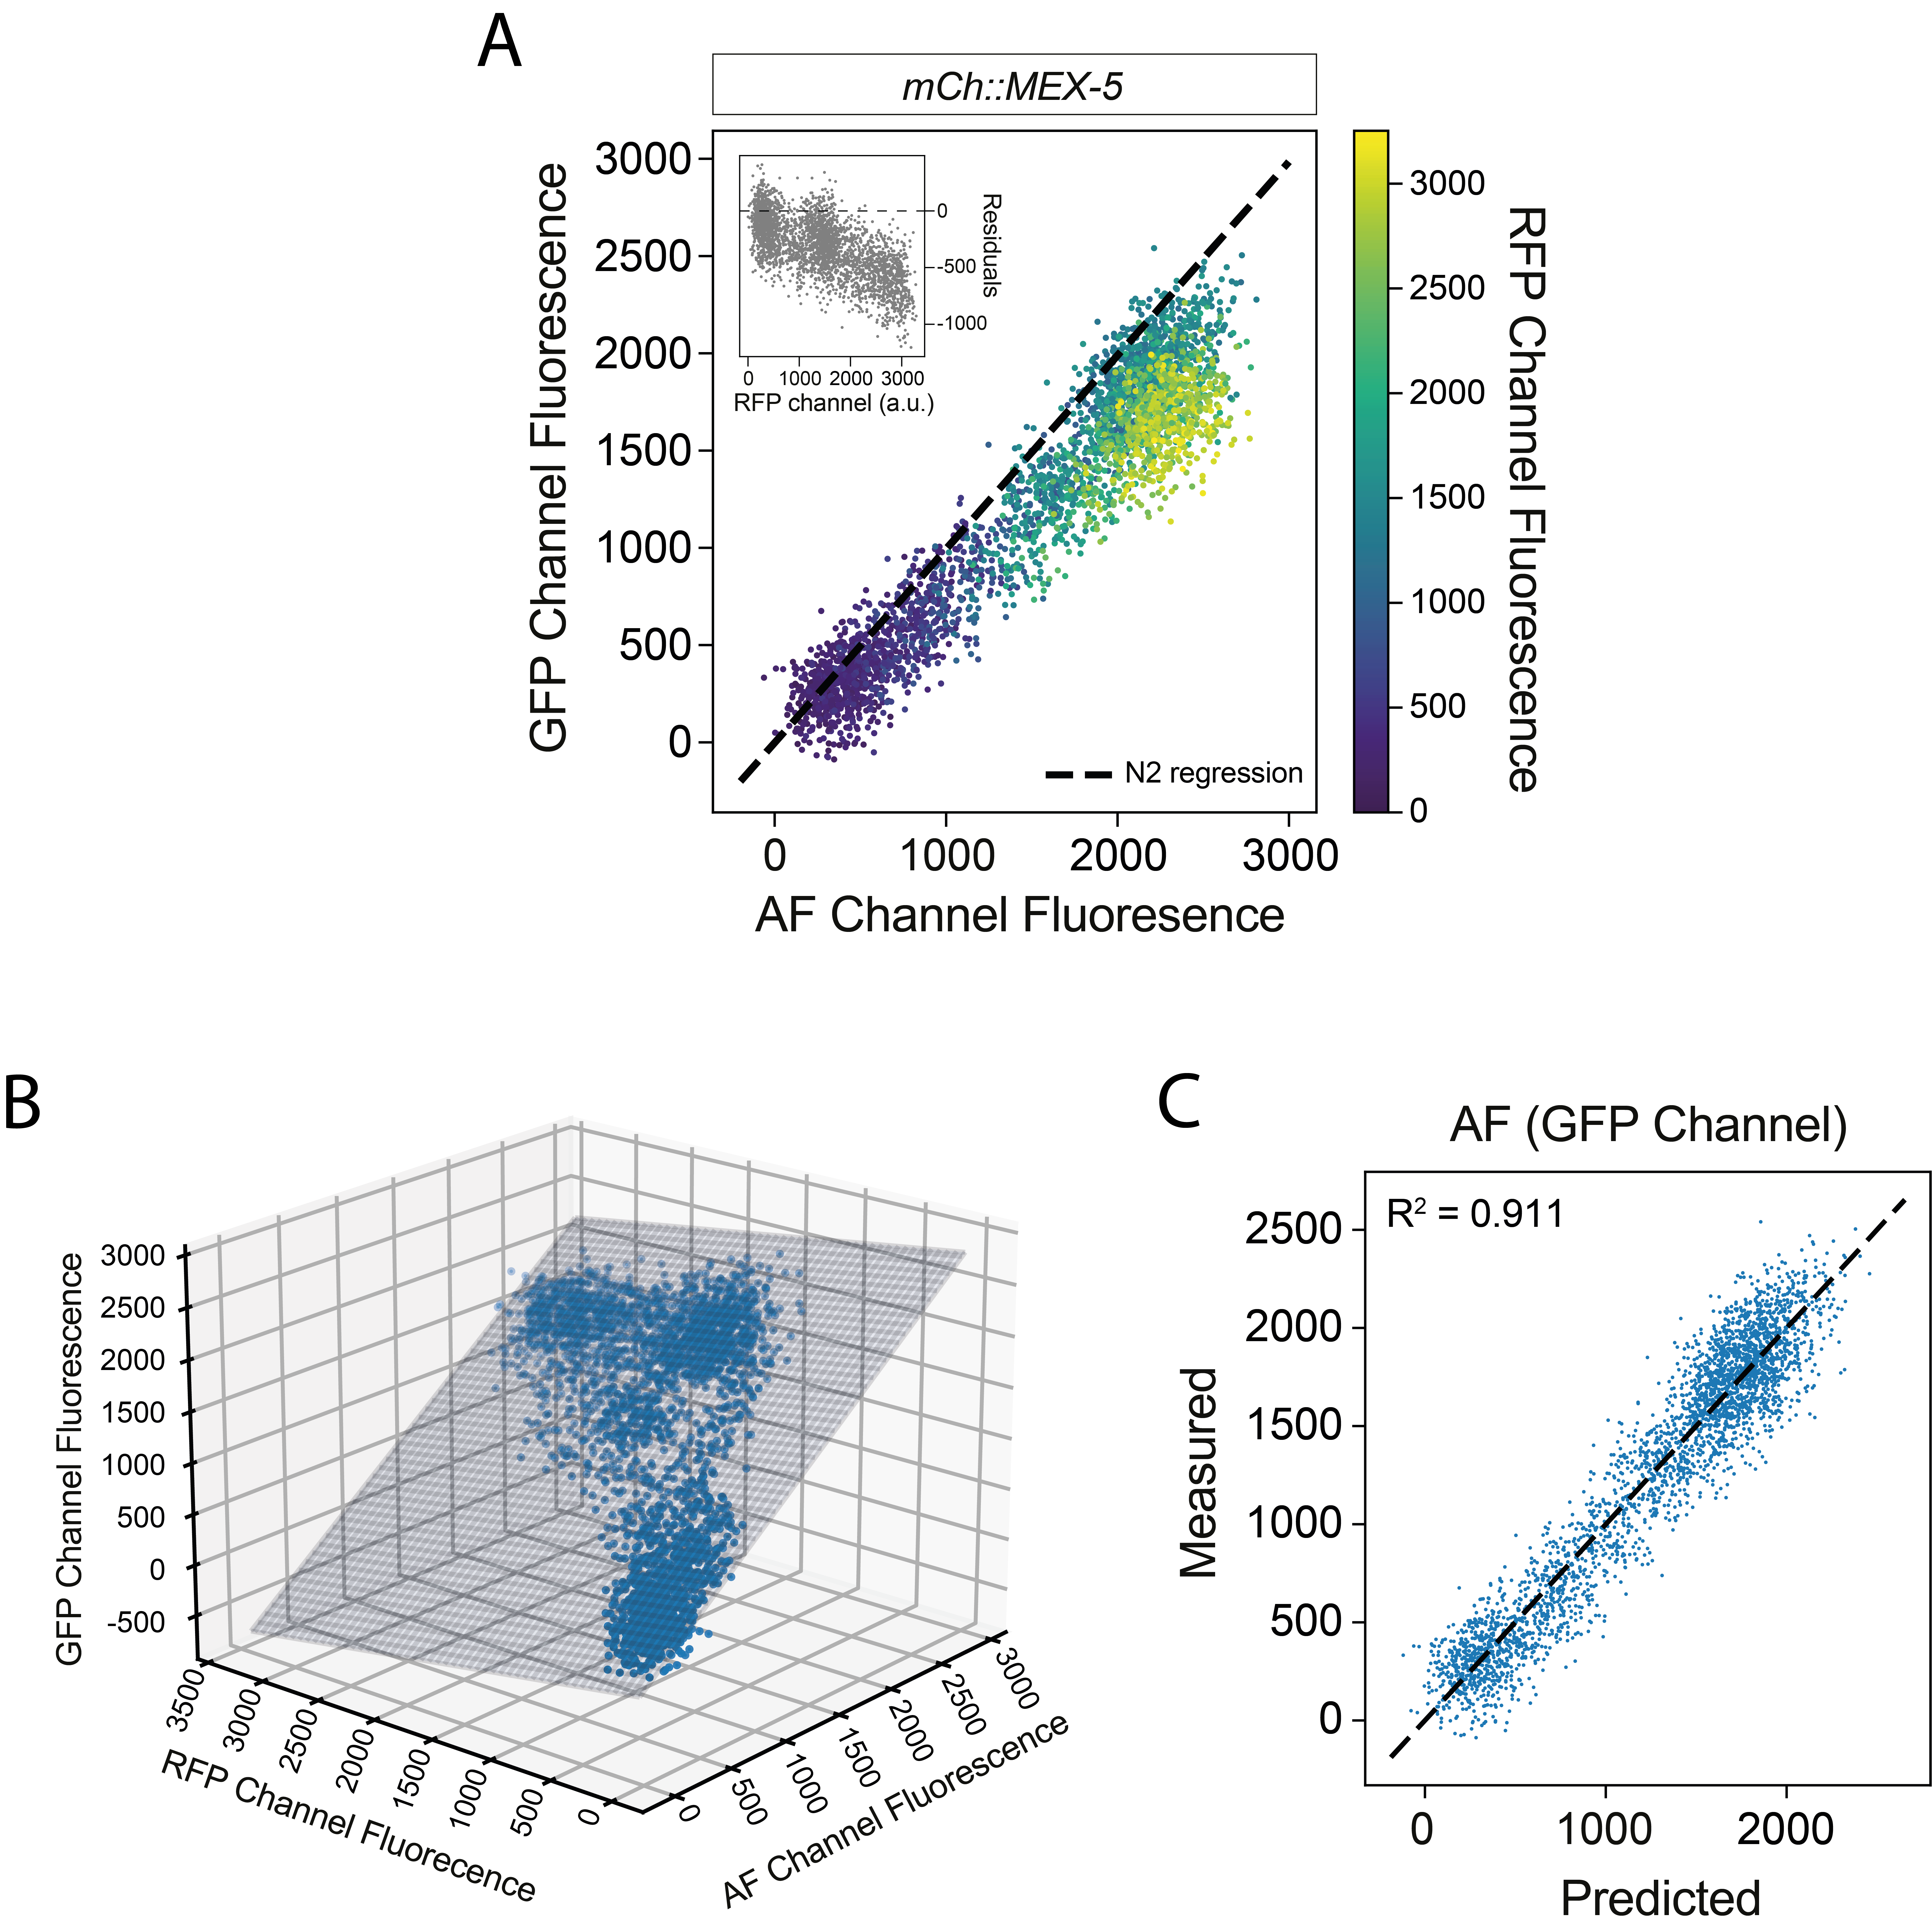
\includegraphics[scale=1]{saibr_3channel_correlation}
\setlength{\abovecaptionskip}{20pt}
\centering
\mycaption{Title}{Caption}
\end{figure}

Then, to perform correction on images containing fluorophore, we just need to capture all three channels, calculate autofluorescence using the three-channel regression relationship obtained from the appropriate RFP tagged single line, and then subtract this away from the GFP channel image. This is demonstrated in figure x, for embryos expressing both PAR-6 GFP and MEX5 mCherry, or just MEX5 cherry. Whereas 2-channel SAIBR results in oversubtraction of autofluorescence (particularly visible in the MEX5 cherry single line), this is eliminated when using 3-channel SAIBR.\\

\begin{figure}[!h]
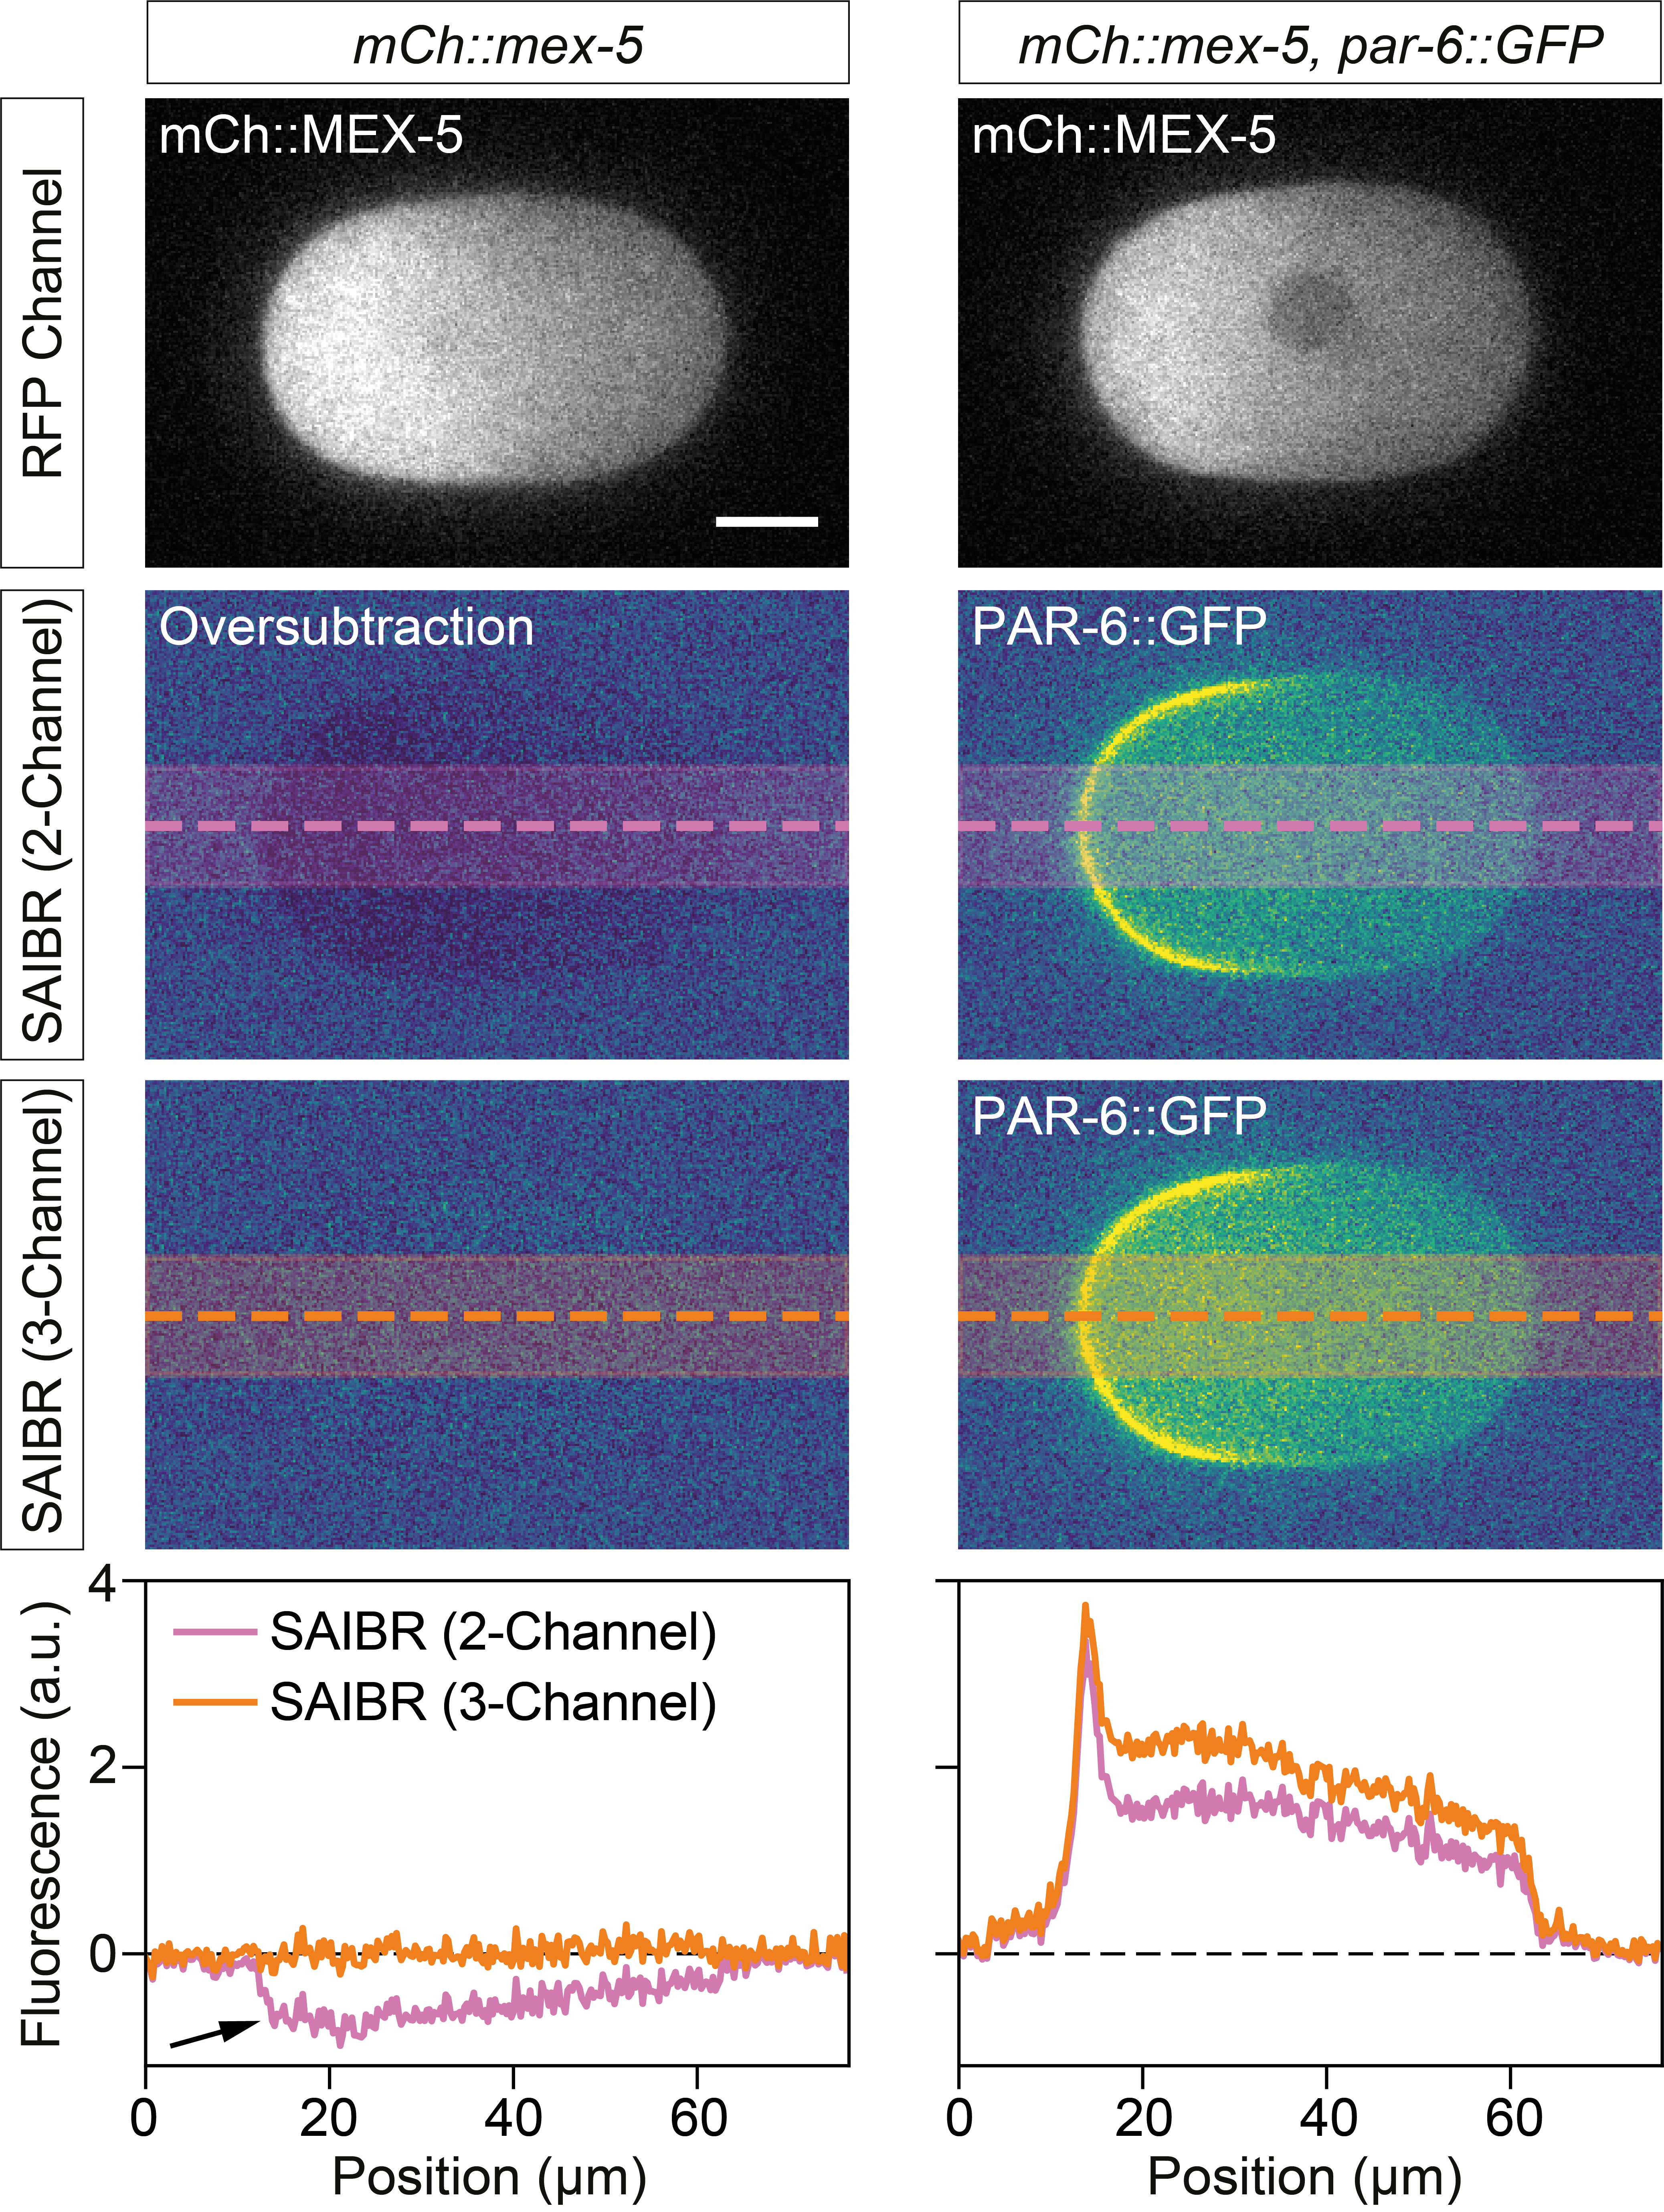
\includegraphics[scale=1]{saibr_3channel_correction}
\setlength{\abovecaptionskip}{20pt}
\centering
\mycaption{Title}{Caption}
\end{figure}


\clearpage
\subsubsection{Discussion}

\clearpage
\subsection{Extraction of membrane and cytoplasmic signal components}

% intro to section

A number of methods have been implemented aiming to quantify cortical protein amounts in C elegans embryos. A typical approach to quantify membrane concentrations is to find the region of the image representing the cortex (either by manual or computational segmentation) and take a coarse measure of pixel values within this region (fig x). Such an approach was used by Goehring, who manually segmented the embryo cortex, computationally straightened a region around the circumference of the cell, and summed the highest intensity group of pixels at each cortical cross section. Hubatsch used a similar approach, but replaced manual segmentation with an automated computational pipeline. Similarly, Zhang used an elaborate computational protocol to segment images, and defined cortical concentrations around the cell as the average signal intensity within a region representing the cortex.\\

% figure: intensity based vs fitting procedures

A main disadvantage of these methods is that, as the cortex is immediately apposed the cytoplasm, pixel values at the cortex will inevitable contain a contribution from cytoplasmic fluorophore signal (and, indeed, cytoplasmic autofluorescence as none of these methods (?) have used spatial autofluorescence correction). This means that measurements of membrane concentration will sensitive the changes in cytoplasmic concentrations, and means that the methods fail to achieve an accurate zero (a positive signal will always register, even if there is nothing on the cortex). Typically, attempts are made to overcome this latter point by normalising concentrations and/or subtracting away a local or global estimate of the background signal, but this is often difficult and inaccurate.\\

More advanced methods have aimed to overcome this problem by building models to describe the expected shape of individual cross-cortex profiles, based on summed contributions of cytoplasmic and membrane signal. Membrane and cytoplasmic concentrations can then be extracted by fitting measured profiles to this model, and extracting the relevant parameters describing the amplitudes of the two signal components (fig x). Such an approach was used by Gross, who described the cross-cortex profile at each point around the circumference of the embryo as the sum of a Gaussian and an error function contribution, representing the expected form of a point (cortex) or step-function (cytoplasm) convolved with a Gaussian-like point spread function in 1D. The model also includes a parameter describing the position of the cortex, which can be optimised to align the model to the profile, eliminating the need for accurate prior segmentation. A similar approach was previously used in Blanchoud (although with a slightly different description of cytoplasmic signal).\\

\subsubsection{Accounting for out-of-focus scatter}

Whilst these methods have been effectively deployed, and are good at capturing a proper zero baseline, their accuracy is inevitably limited by the accuracy of the underlying models. For many imaging set-ups, the assumption that cytoplasmic and membrane contributions can be described by such simple mathematical functions may in fact be far from the truth. This was demonstrated by Reich, who quantitatively analysed cross-cortex signal in cells containing only cytoplasmic protein, finding that (under imaging conditions similar to those used in this study) the shape of this profile deviates significantly from the expected error-function shape.\\

% * can be seen in figure A.3 of Jake’s thesis, although it’s worth noting that the original study didn’t use spatial autofluorescence correction, so there may be some artefacts relating to this

% description of cytbg figure

% cytbg figure

The main reason for this is likely due to scattering and diffraction of light from planes above and below the imaging plane, combined with a curved geometry in the z-dimension (fig x). Scatter, which is a common issue in images of biological samples, is a broadening of light in three dimensions as it passes through regions of heterogeneous refractive index. This occurs within the (xy) plane of an image, but is typically far more significant in the z-plane. Whilst confocal microscopes are designed to only capture light from a single plane, they illuminate the whole sample, so will capture any emitted light from other planes that scatters into the focal plane. This means that pixel intensities within the focal plane will be affected not only by structures within that plane but also structures above and below.\\



\begin{figure}[!h]
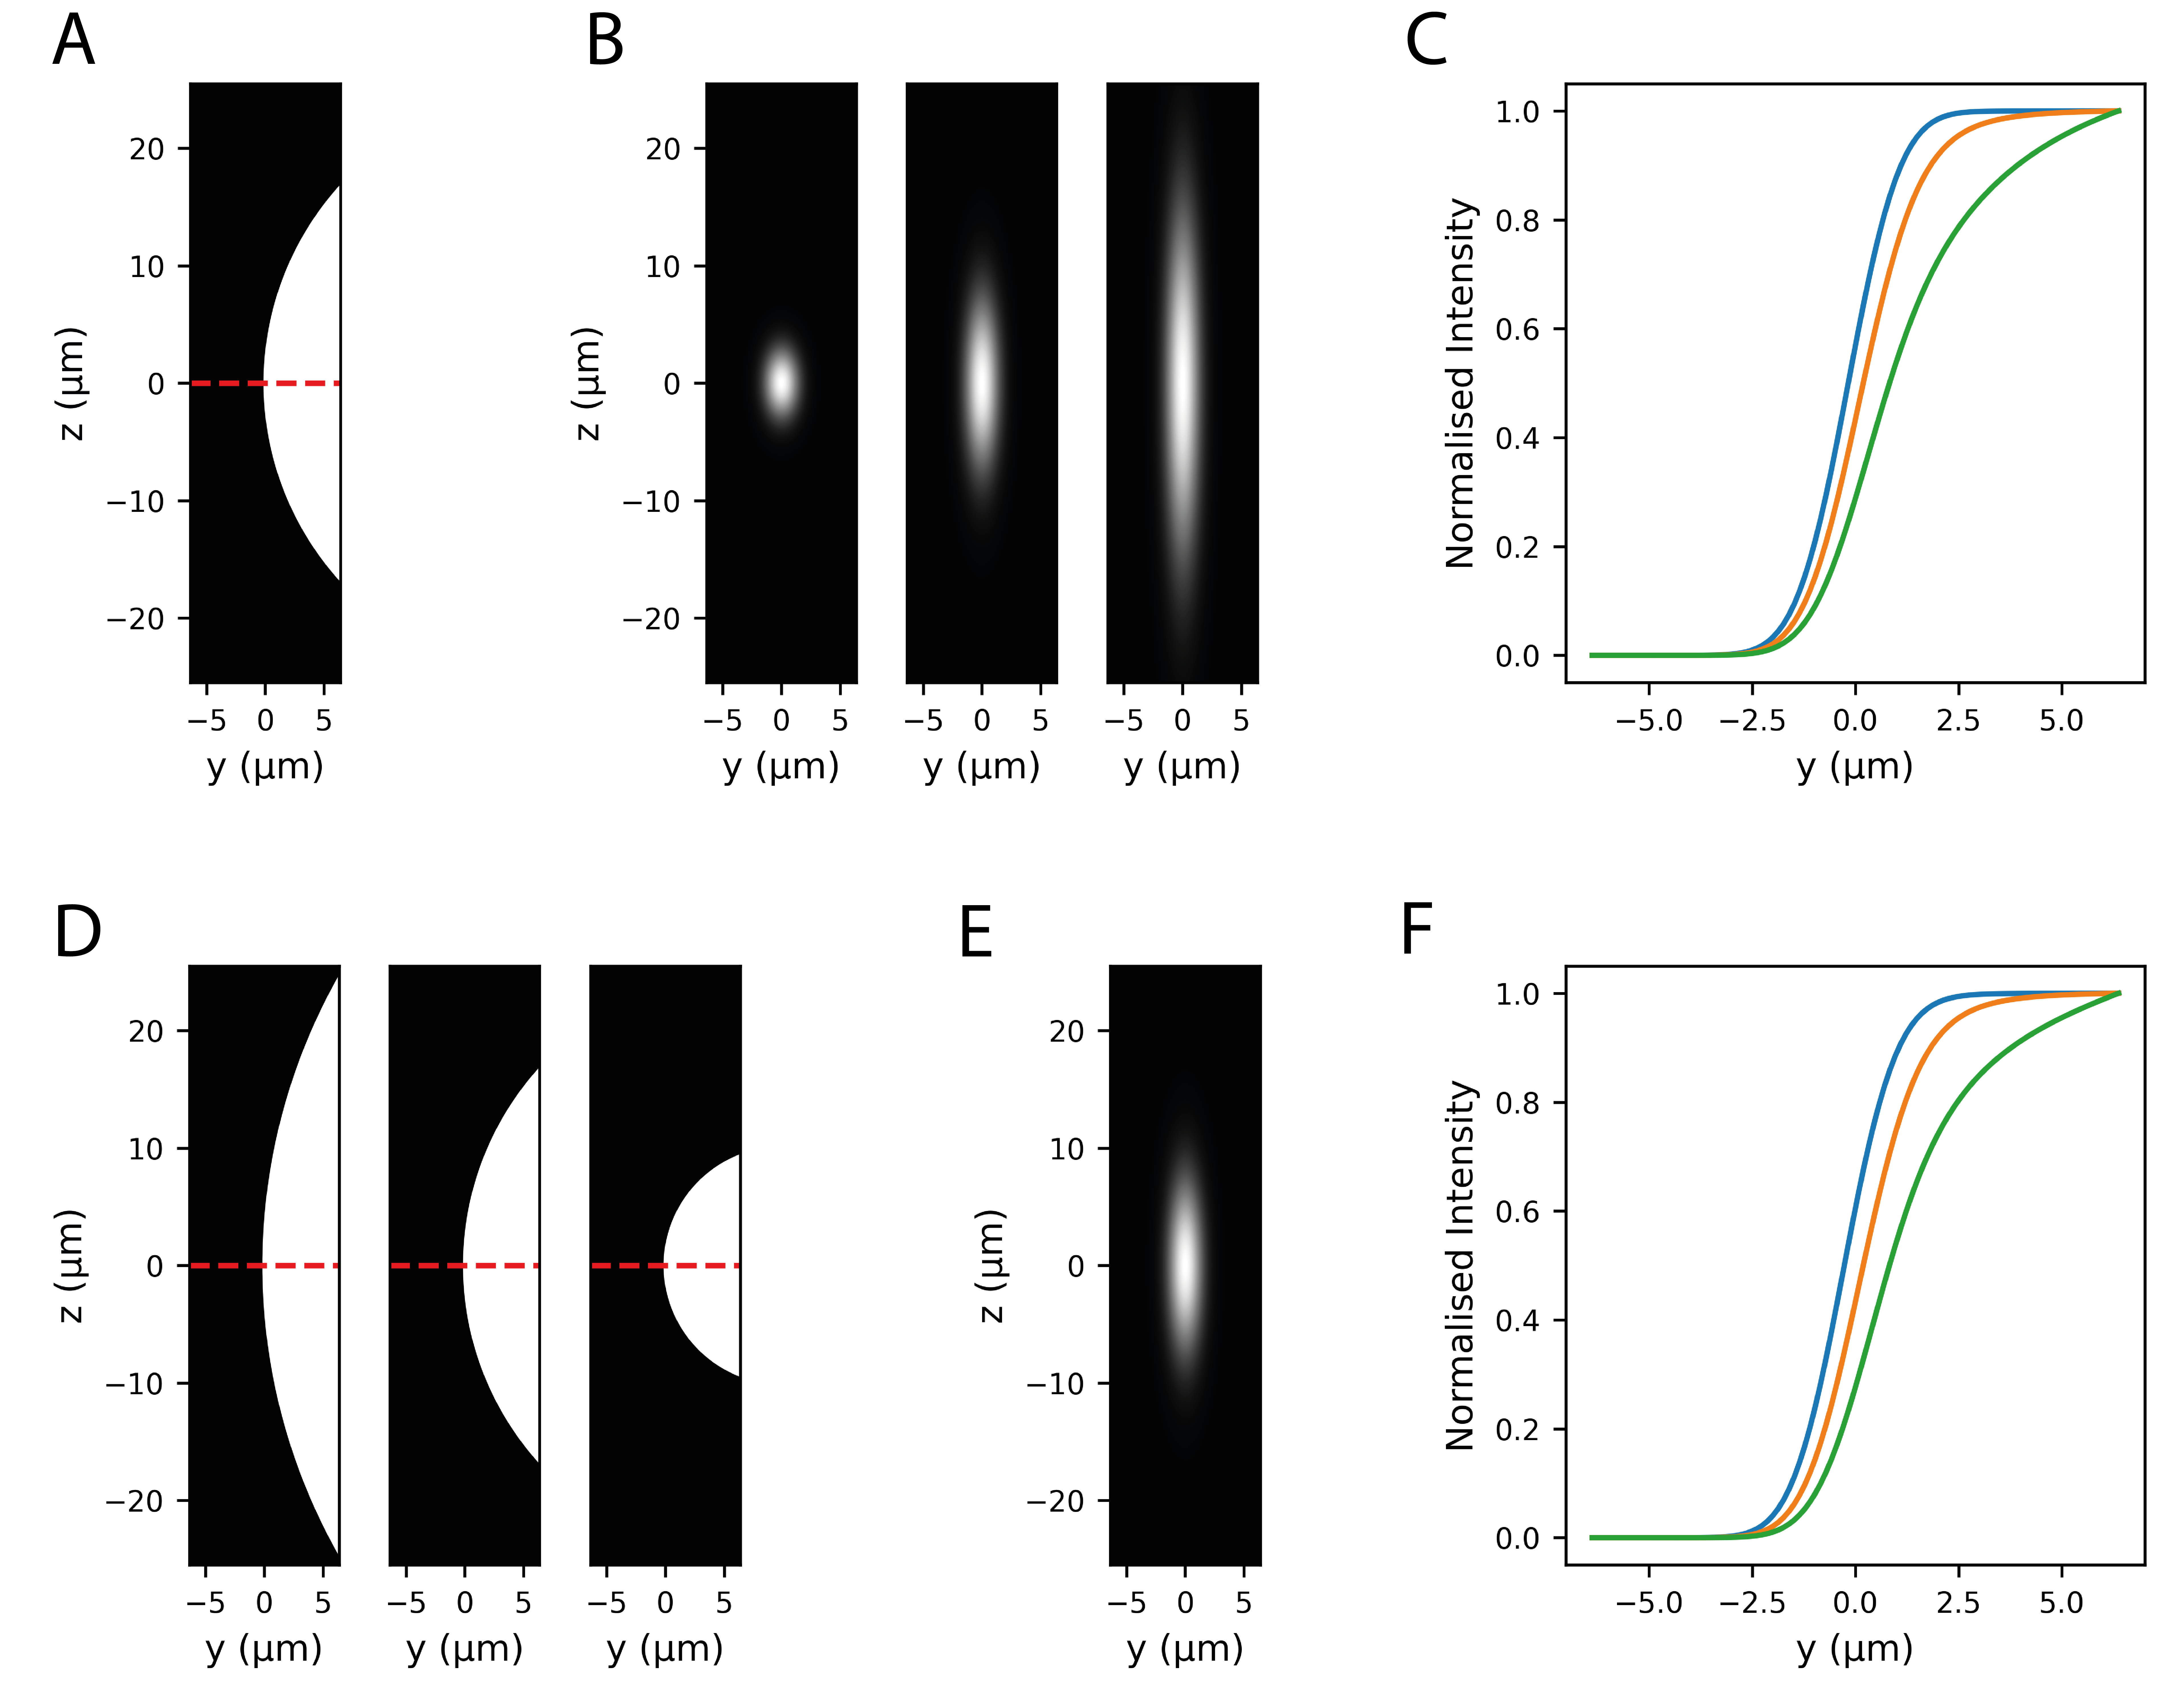
\includegraphics[scale=0.9]{memquant_cyt_psf}
\setlength{\abovecaptionskip}{20pt}
\centering
\mycaption{Title}{Caption}
\end{figure}

It is likely that a similar problem applies in the case of membrane protein (fig x). Specifically, this analysis shows that out of focus cortical signal might expect to lead to a shape resembling an asymmetric Gaussian, with higher signal on the inside than the outside. In fact, this phenomenon can be easily observed just by looking at images of polarised PAR proteins (<reference earlier image>), where out-of-focus cortical signal can create the illusion of a strong cytoplasmic gradient (by comparison, two-photon images of PAR-2, which aim to eliminate out of focus light, show a completely flat cytoplasm (Petrasek), which is expected for most PAR proteins based on fast measured diffusion rates). Whilst in some cases this may be of little concern, this might be particularly problematic if accurate cytoplasmic quantification is required. Without accurate cytoplasmic concentration, measures of membrane to cytoplasmic ratio, which is often used as a proxy for membrane affinity (see later section), may be wildly off. This will prove significant for much of the analysis in this study.\\

\begin{figure}[!h]
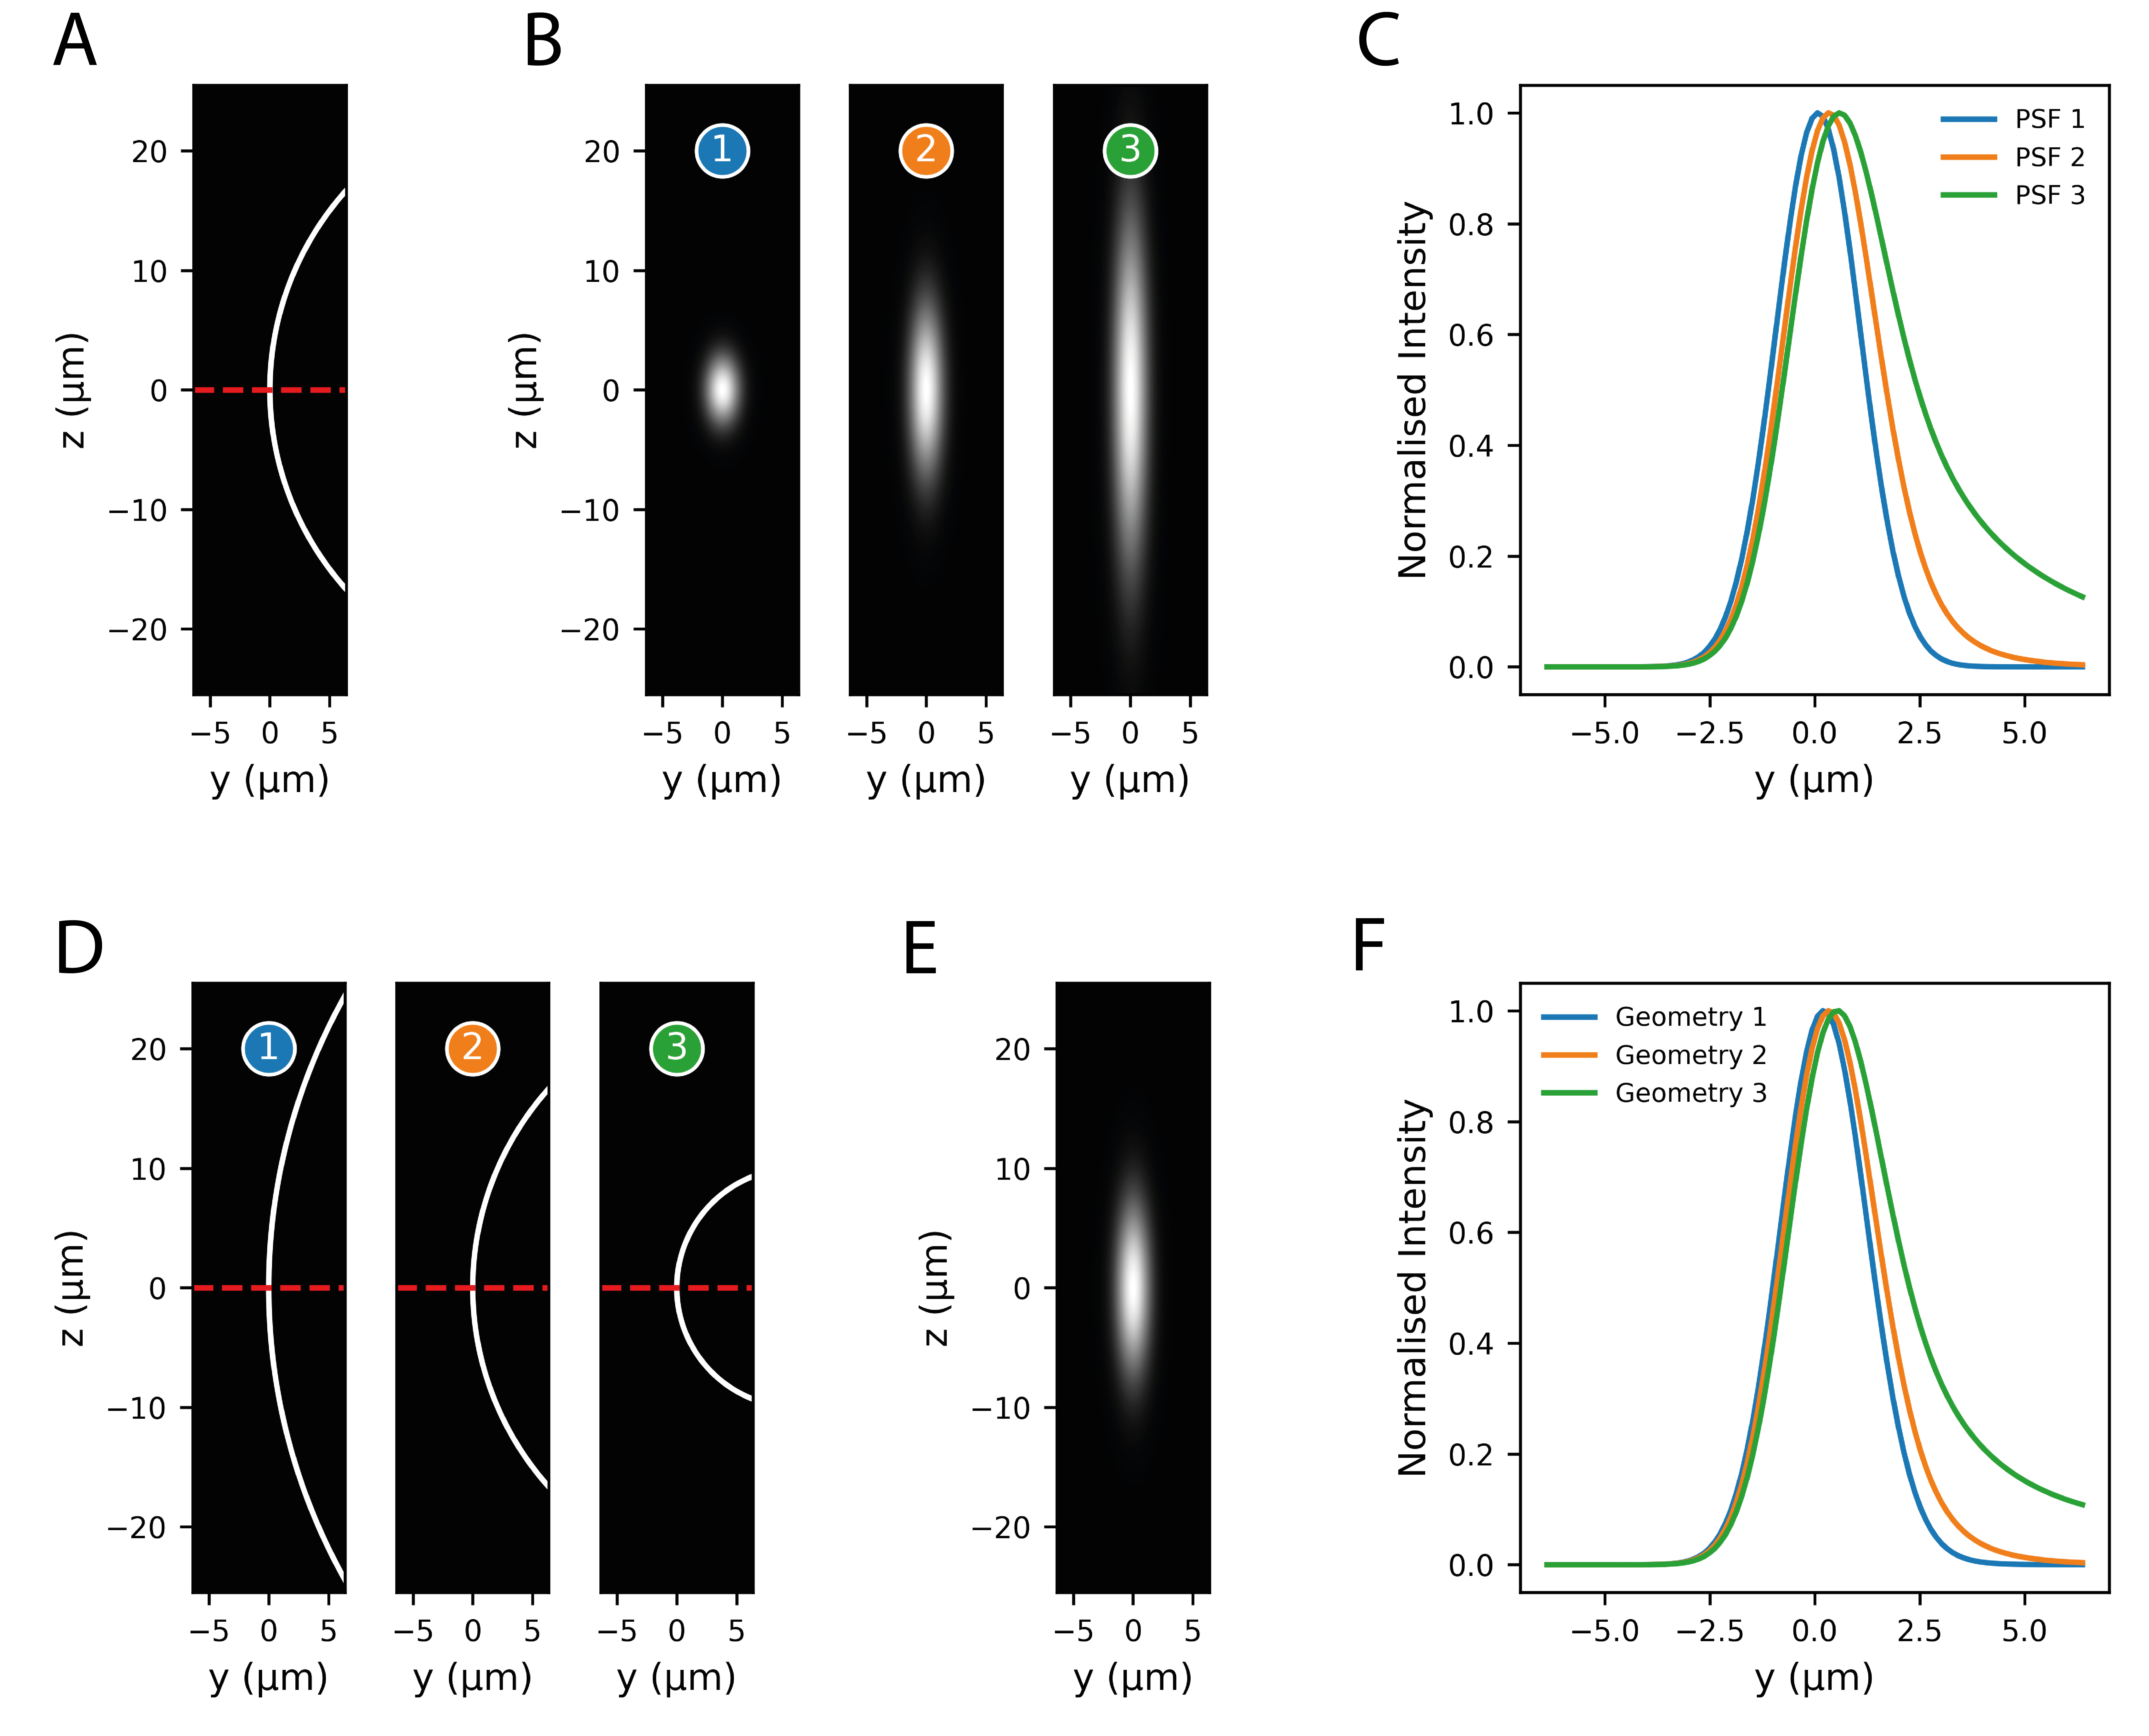
\includegraphics[scale=0.9]{memquant_mem_psf}
\setlength{\abovecaptionskip}{20pt}
\centering
\mycaption{Title}{Caption}
\end{figure}

Typically, one might account for out-of-focus scatter by taking a z-stack from across the whole sample, and applying a deconvolution algorithm to the 3D stack to reassign all blurred/scattered light to an in-focus location (Wallace). These methods rely on prior knowledge of the point spread function that applies to the particular sample and imaging set-up, which needs to be as accurate as possible, otherwise artefacts can result. Theoretical methods exist to estimate an appropriate PSF given parameters such as the imaging modality, numerical aperture and emitted light wavelength. Whilst these methods are good at describing blur within the imaging apparatus, scattering within the sample and at the sample-apparatus interface is difficult to model. For this reason, it can be more effective to measure an empirical PSF by imaging the light distribution from a single point source (e.g. a fluorescent bead) under similar sample prep conditions to your sample of interest. However, as PSFs are influenced by scatter within the sample itself, the accuracy of this method depends on how closely the sample environment can be replicated when imaging the beads, which is difficult. <soaking tissue with beads>.\\

Furthermore, most deconvolution methods assume that the PSF is a constant function throughout the whole image, but in many cases this won't be the case. There may, for example, be refractive index gradients within the sample, which alter the shape of the PSF depending on location within the sample. Additionally, if there is a mismatch between the refractive index of the immersion and mounting media, as is often unavoidable when imaging live biological samples, then the PSF will vary with depth as spherical aberrations will be introduced deeper into the sample. A PSF from a fluorescent bead located directly below the coverslip will not capture either of these phenomena.\\

In reality, given all of these confounding factors, an accurate description of the PSF that applies to a given sample of interest is often an unachievable goal. Whilst deconvolution with a suboptimal PSF may be sufficient for many qualitative applications, accurate quantitative measurements cannot be guaranteed. For this reason, I opted against using a deconvolution approach to account for out-of-plane scattering.\\

% transition

%in most cases it should be possible to predict the distribution of protein in planes above and below based on the midplane image

As the normalised shape of this profile is a function only of local embryo geometry and the optical properties of the microscope/sample, both of which should be largely consistent from point to point around the circumference, and from embryo to embryo, an explicit description of light scattering is not necessary, and it should be sufficient to rely on a phenomenological description of the cytoplasmic and membrane signal contributions. Reich exploited this idea by replacing the error-function description of cytoplasmic signal with his arbitrary, measured, cytoplasmic reference profile, thus describing the total signal as the sum of a Gaussian profile and this arbitrary profile. The result was a far better ability of the model to fit the shape of measured profiles.\\

Whilst this move is a significant step in the right direction, the problem remains of how best to account for out of focus cortical light. This presents a challenge: whilst it is relatively easy to directly measure a cytoplasmic reference profile (you just need a reference image in which all signal is cytoplasmic), the same is not true for a membrane profile as it is difficult/impossible to find a reference case in which all protein is membrane bound. \\

%<Eggshell method> An initial idea, involving staining of the exterior of the eggshell with a fluorescent dye proved technically challenging and not reproducible.

% introduce ideas here - uniform cytoplasm so contribution can be predicted

\clearpage
\subsubsection{A gradient descent protocol for image quantification}

\begin{figure}[!h]
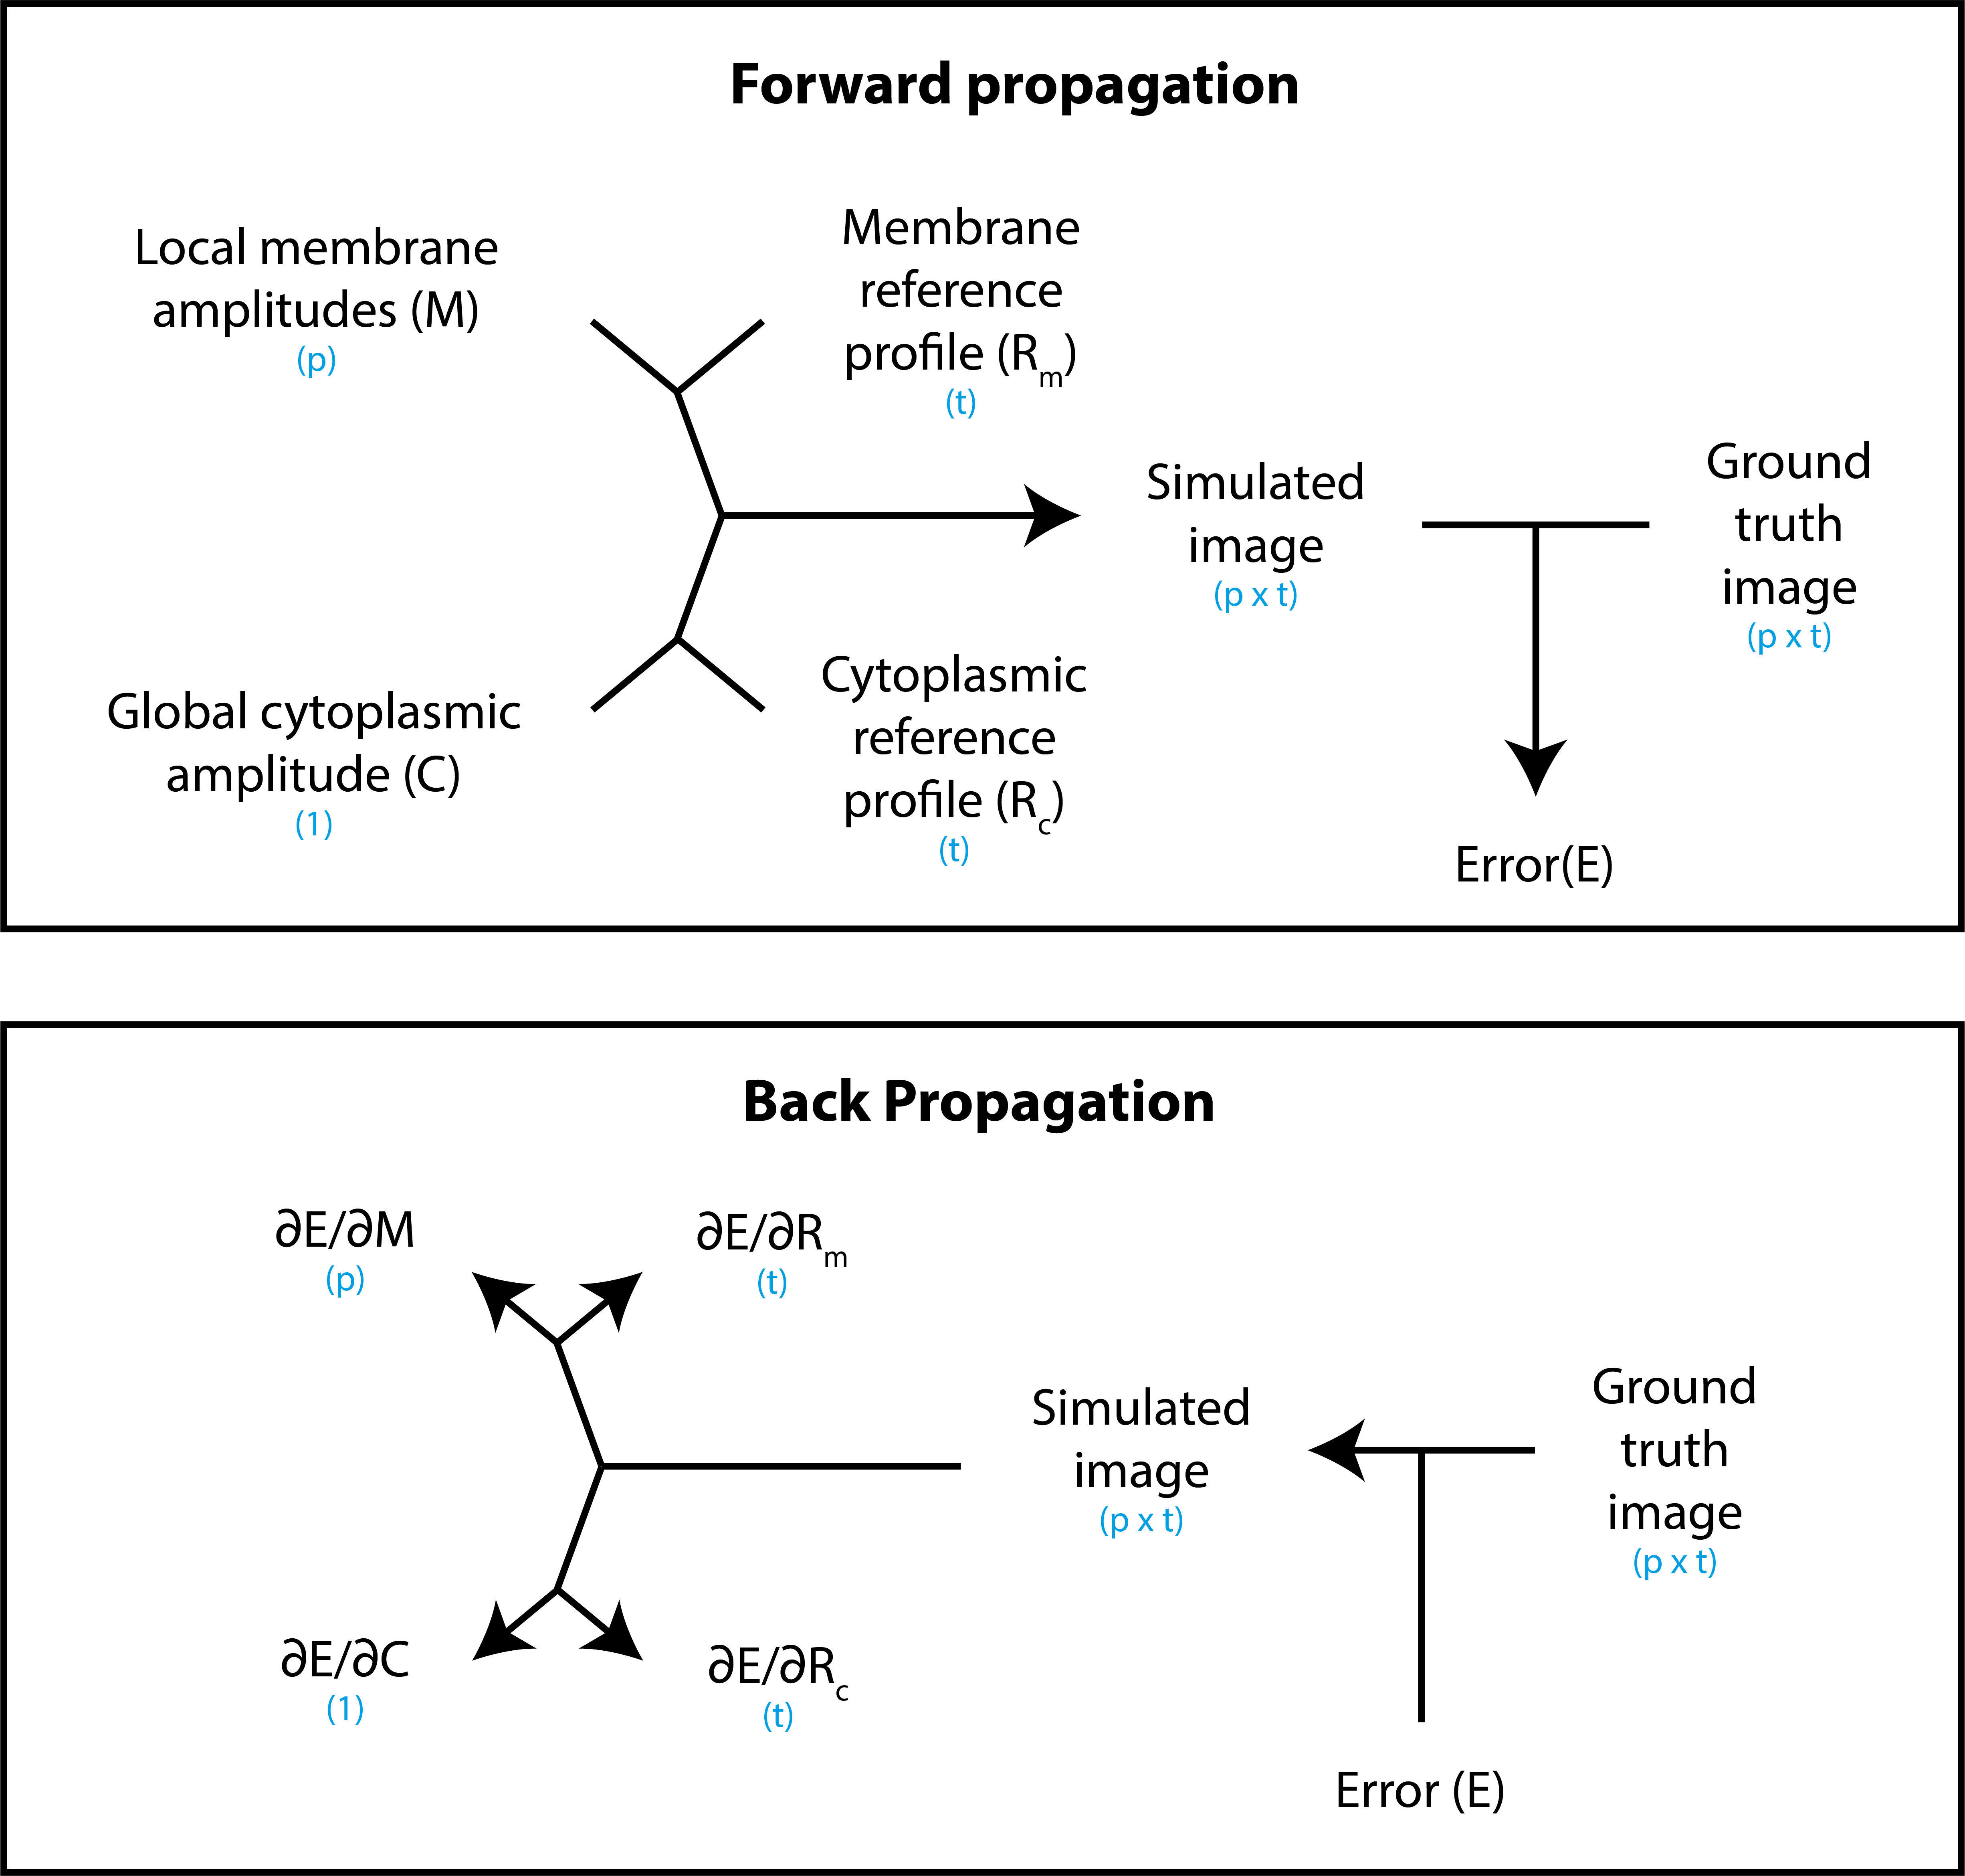
\includegraphics[scale=1]{memquant_forward_and_back_propagation}
\setlength{\abovecaptionskip}{20pt}
\centering
\mycaption{Title}{Caption}
\end{figure}

\begin{figure}[!h]
\includegraphics[scale=1]{memquant_membg_training}
\setlength{\abovecaptionskip}{20pt}
\centering
\mycaption{Title}{Caption}
\end{figure}

\clearpage
\subsubsection{Segmentation}

A nice outcome of this is that the offset parameters can then be used to refine the original ROI. As a result, initial ROIs need only be very rough (4 haphazard clicks around the cortex generally suffices, compared to ~20 which may be required to accurately trace the cortex).\\


\clearpage
\subsubsection{Benchmarking the method}

\begin{figure}[!h]
\includegraphics[scale=1]{memquant_benchmarking_ph_rundown}
\setlength{\abovecaptionskip}{20pt}
\centering
\mycaption{Title}{Caption}
\end{figure}

\begin{figure}[!h]
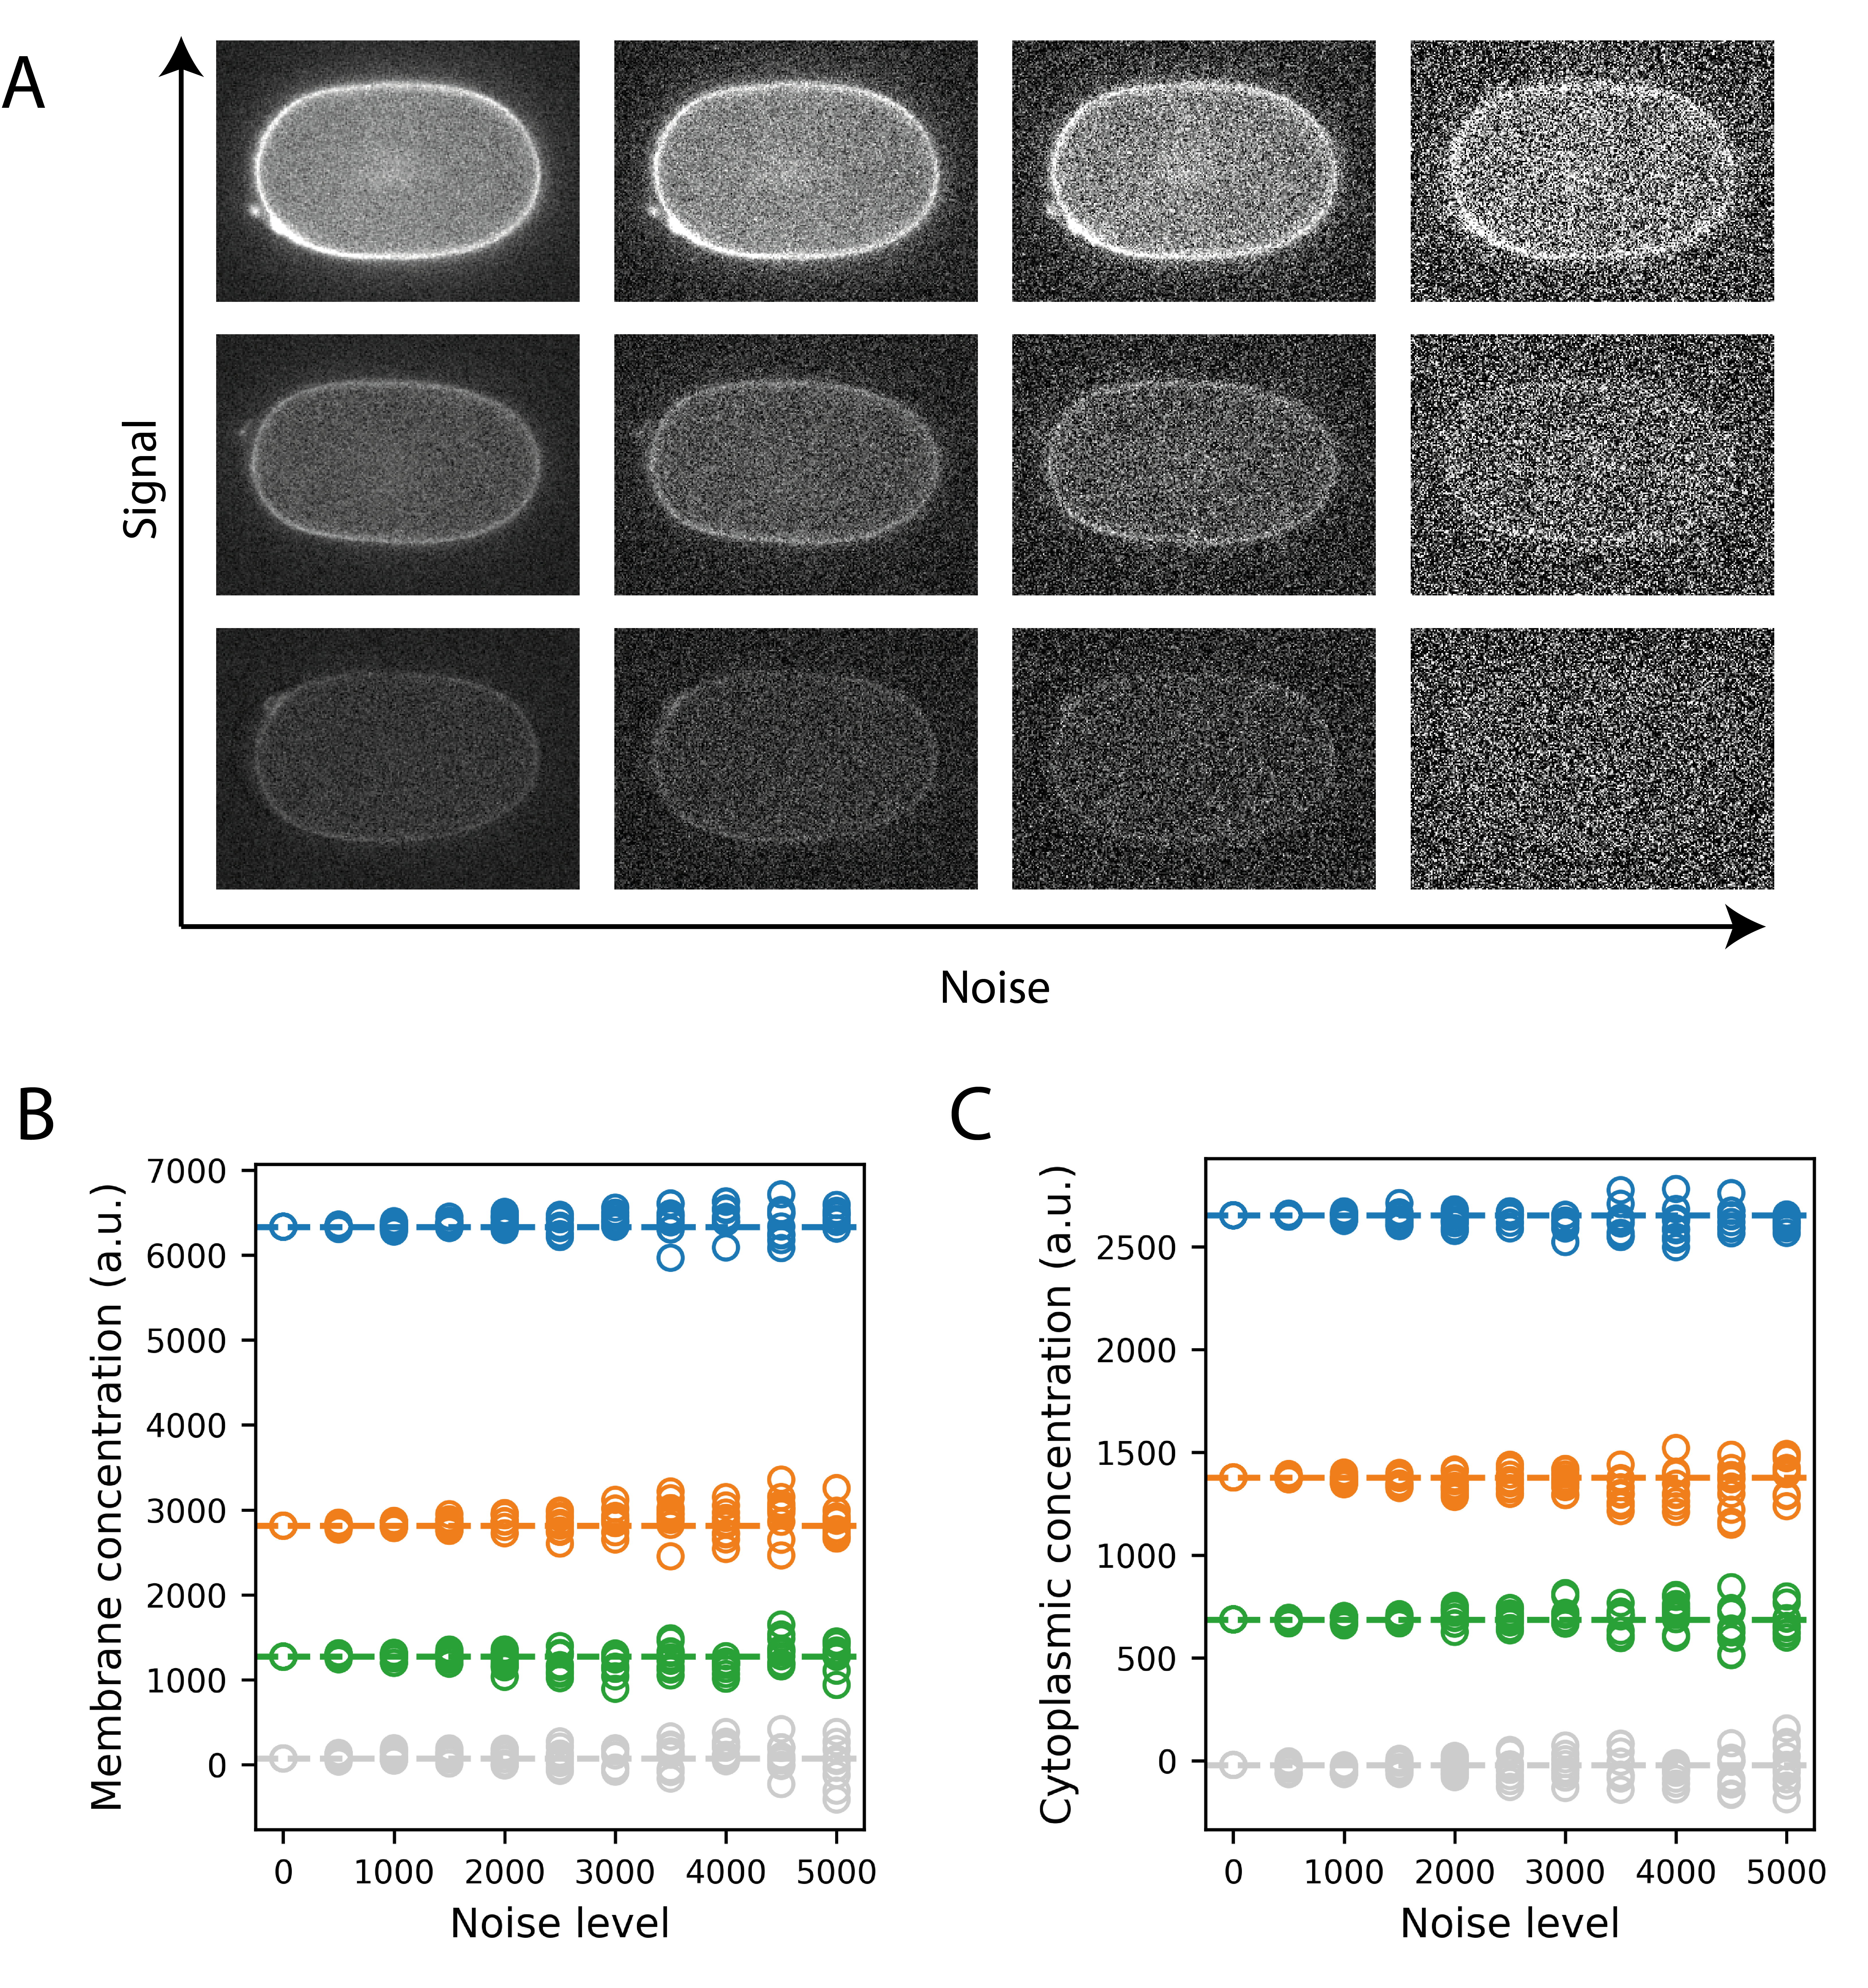
\includegraphics[scale=0.9]{memquant_benchmarking_noise}
\setlength{\abovecaptionskip}{20pt}
\centering
\mycaption{Title}{Caption}
\end{figure}


\clearpage
\subsubsection{Calibration of concentration units}

%taken from tc3 - need to modify to match format of the thesis
As $\alpha$ and $\beta$ are unitless constants, a conversion parameter, c, is required. To calibrate this conversion parameter, I quantified the effects on $\alpha$ and $\beta$ measurements of redistributing a fixed pool of protein from the cytoplasm to the cortex. To do this, I used an optogenetics system with a membrane bound PH::eGFP::LOV to move a cytoplasmic pool of ePDZ::mCherry to the membrane (Fielmich et al., 2018). Embryos were exposed to a xxxx, which promotes binding between ePDZ and LOV, leading to a rapid uniform recruitment of ePDZ::mCherry to the membrane and a reduction in the concentration in the cytoplasm. Assuming a fixed dosage of ePDZ::mCherry before and after exposure to green light (and negligible mCherry photobleaching), a value of the conversion parameter, $c$, can be calculated for each embryo using equation \ref{eq:c}, giving an estimate of $x \pm x$ (n=x) for $c$.

\begin{equation}
c = \frac{\alpha_{pre \textrm{-} exposure} - \alpha_{post  \textrm{-} exposure}}{\psi (\beta_{post  \textrm{-} exposure} - \beta_{pre  \textrm{-} exposure})}
\label{eq:c}
\end{equation}\\

\begin{figure}[!h]
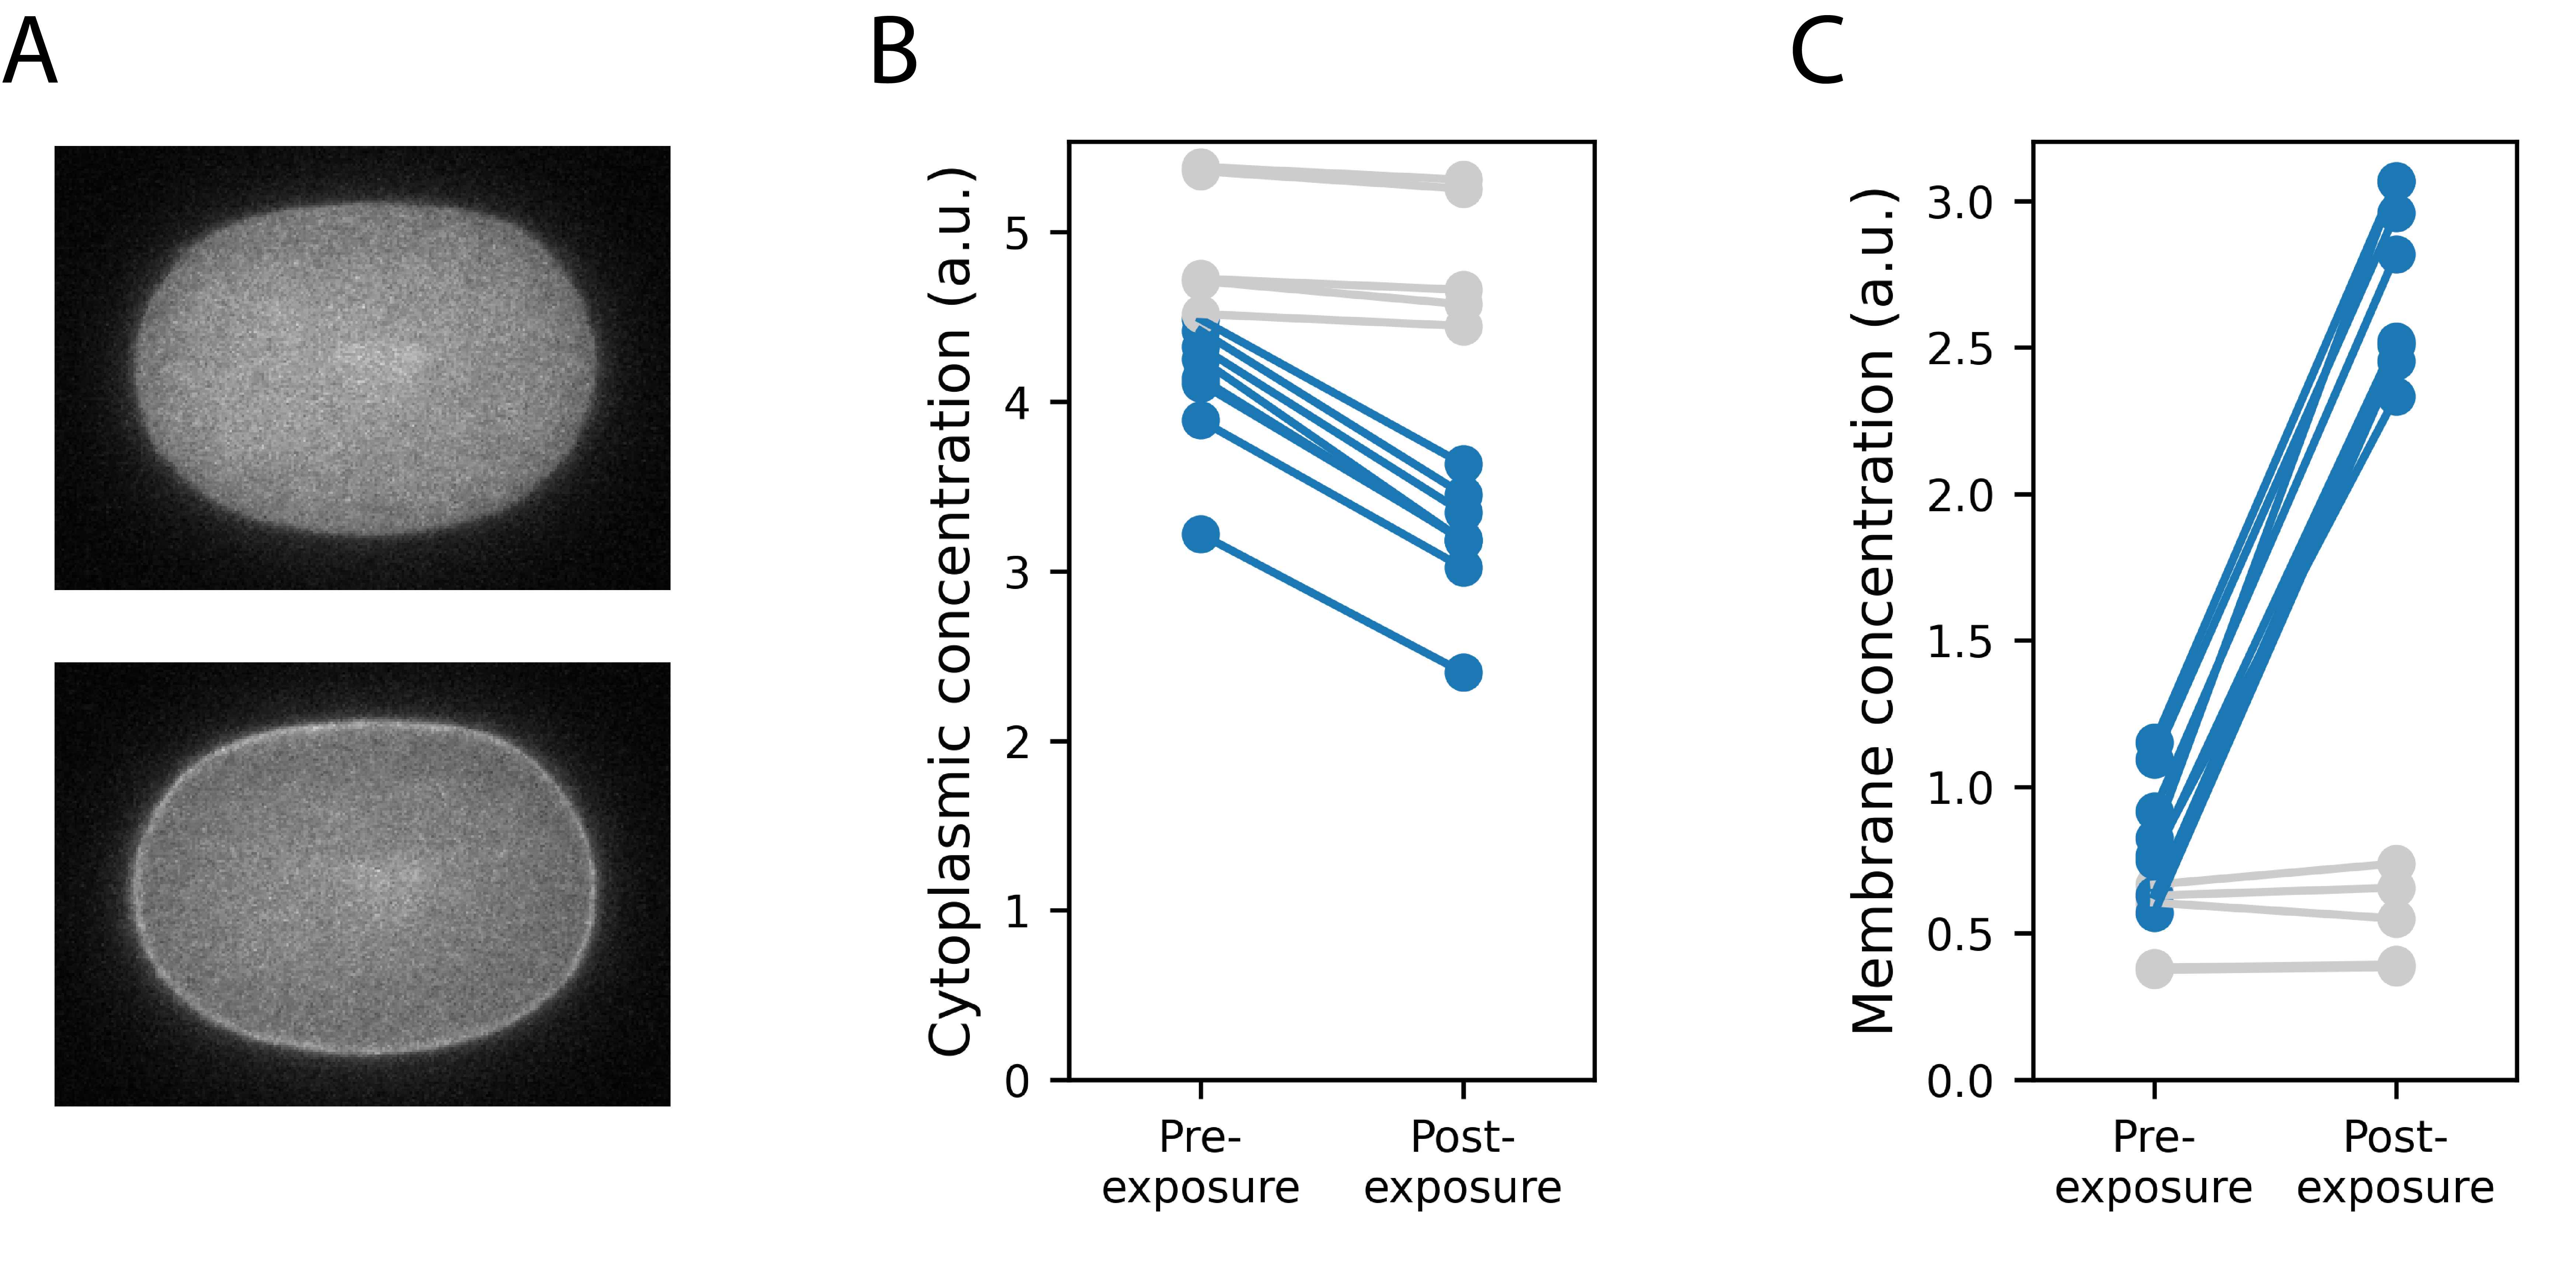
\includegraphics[scale=1]{memquant_optogenetics}
\setlength{\abovecaptionskip}{20pt}
\centering
\mycaption{Title}{Caption}
\end{figure}

\clearpage
\subsubsection{Discussion}

%%%%%%%%%%%%%%%%%%%%%%%%%%%%%%%%%%%%%%%%%%%%%%%%%%%%%%%%%%
\clearpage
\section{Identifying core patterning behaviours of PAR-2}

Text

\subsection{PAR-2 polarity in systems with uniform aPAR}

\subsection{Polarity phenotypes in PAR-2 mutants}

\subsection{Quantitative characterisation of PAR-2 mutants}

\subsection{Discussion}

%%%%%%%%%%%%%%%%%%%%%%%%%%%%%%%%%%%%%%%%%%%%%%%%%%%%%%%%%%
\clearpage
\section{Determining the mechanisms of PAR-2 RING domain action}

Text

\subsection{Exploring a role for ubiquitination}
\subsubsection{PAR-2 purification and in vitro ubiquitination assays}
\subsubsection{Sequence analysis and targeted mutation of putative linchpin site}

\subsection{Exploring a role for dimerisation}
\subsubsection{Structure prediction}
\subsubsection{Characterising dimerisation in vitro}
\subsubsection{Characterising dimerisarion in vivo}
\subsubsection{Targeted mutation to dimerisation interface regions}

\subsection{Discussion}


%%%%%%%%%%%%%%%%%%%%%%%%%%%%%%%%%%%%%%%%%%%%%%%%%%%%%%%%%%
\clearpage
\section{A thermodynamic model of PAR-2 dimerisation}

Text

\subsection{Model description}

\begin{figure}[!h]
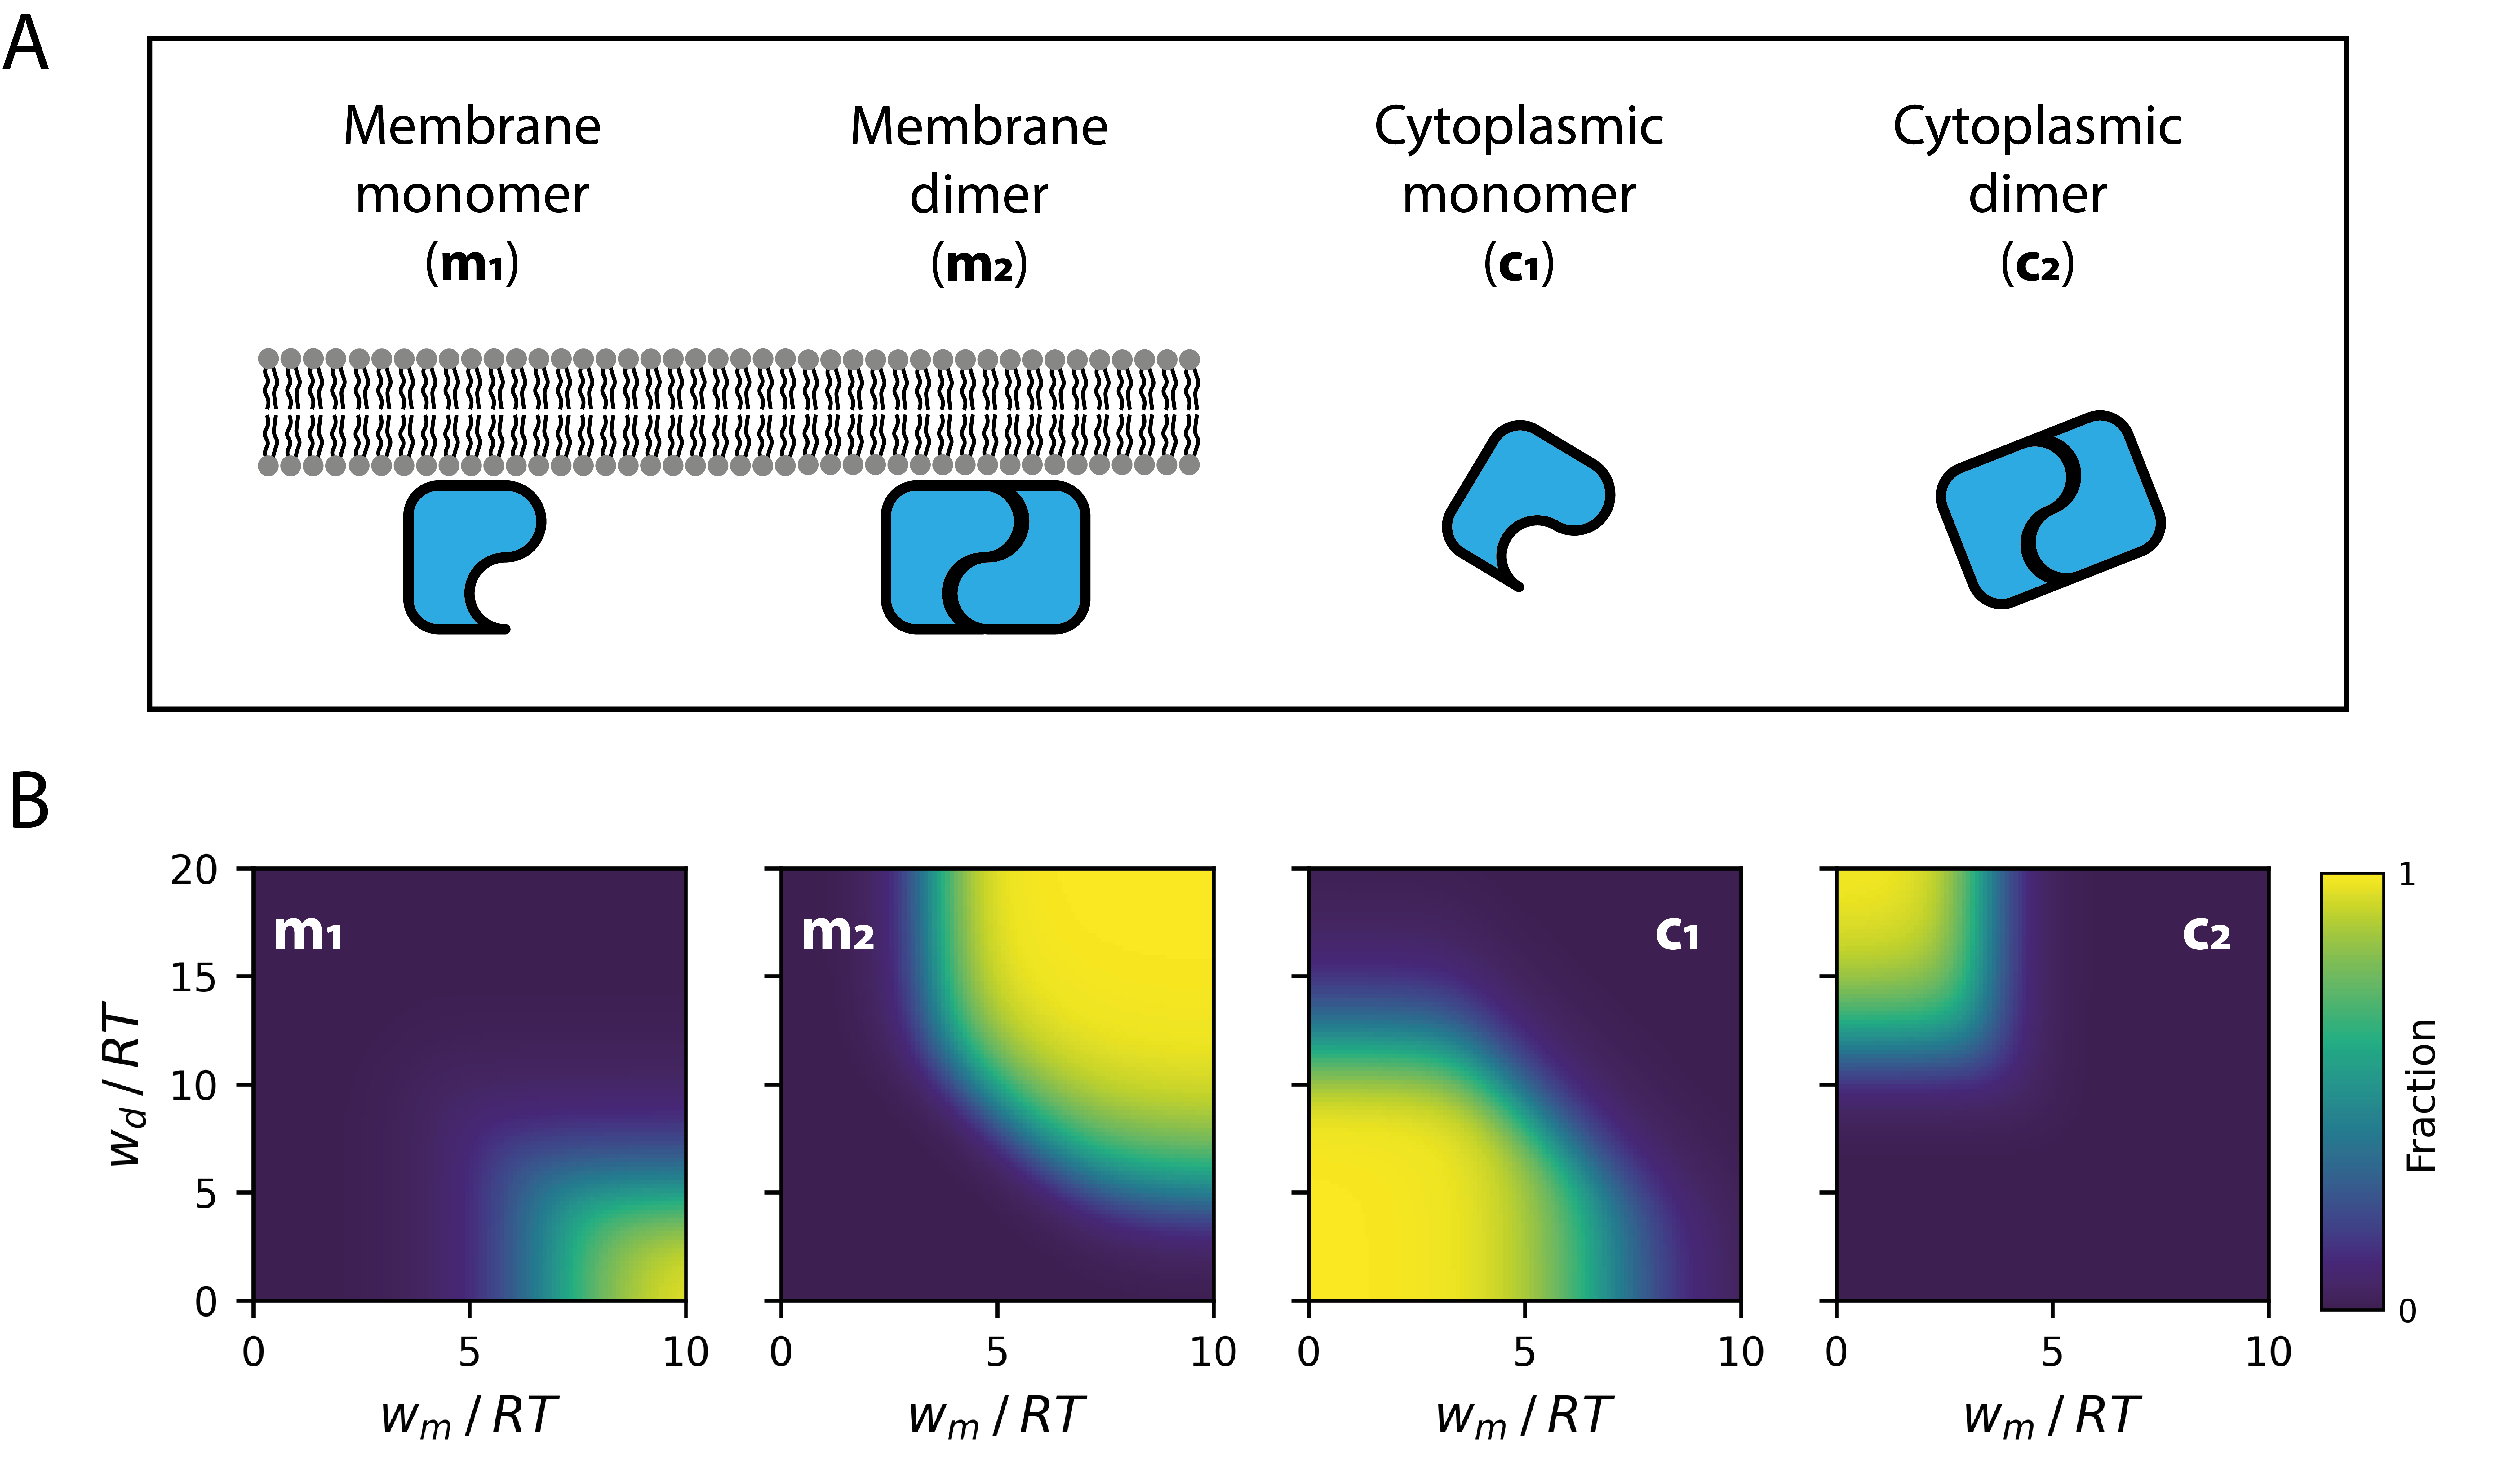
\includegraphics[scale=0.9]{thermodynamic_model_species}
\setlength{\abovecaptionskip}{20pt}
\centering
\mycaption{Title}{Caption}
\end{figure}

\clearpage
\subsection{Dimerisation-driven positive feedback}

\begin{figure}[!h]
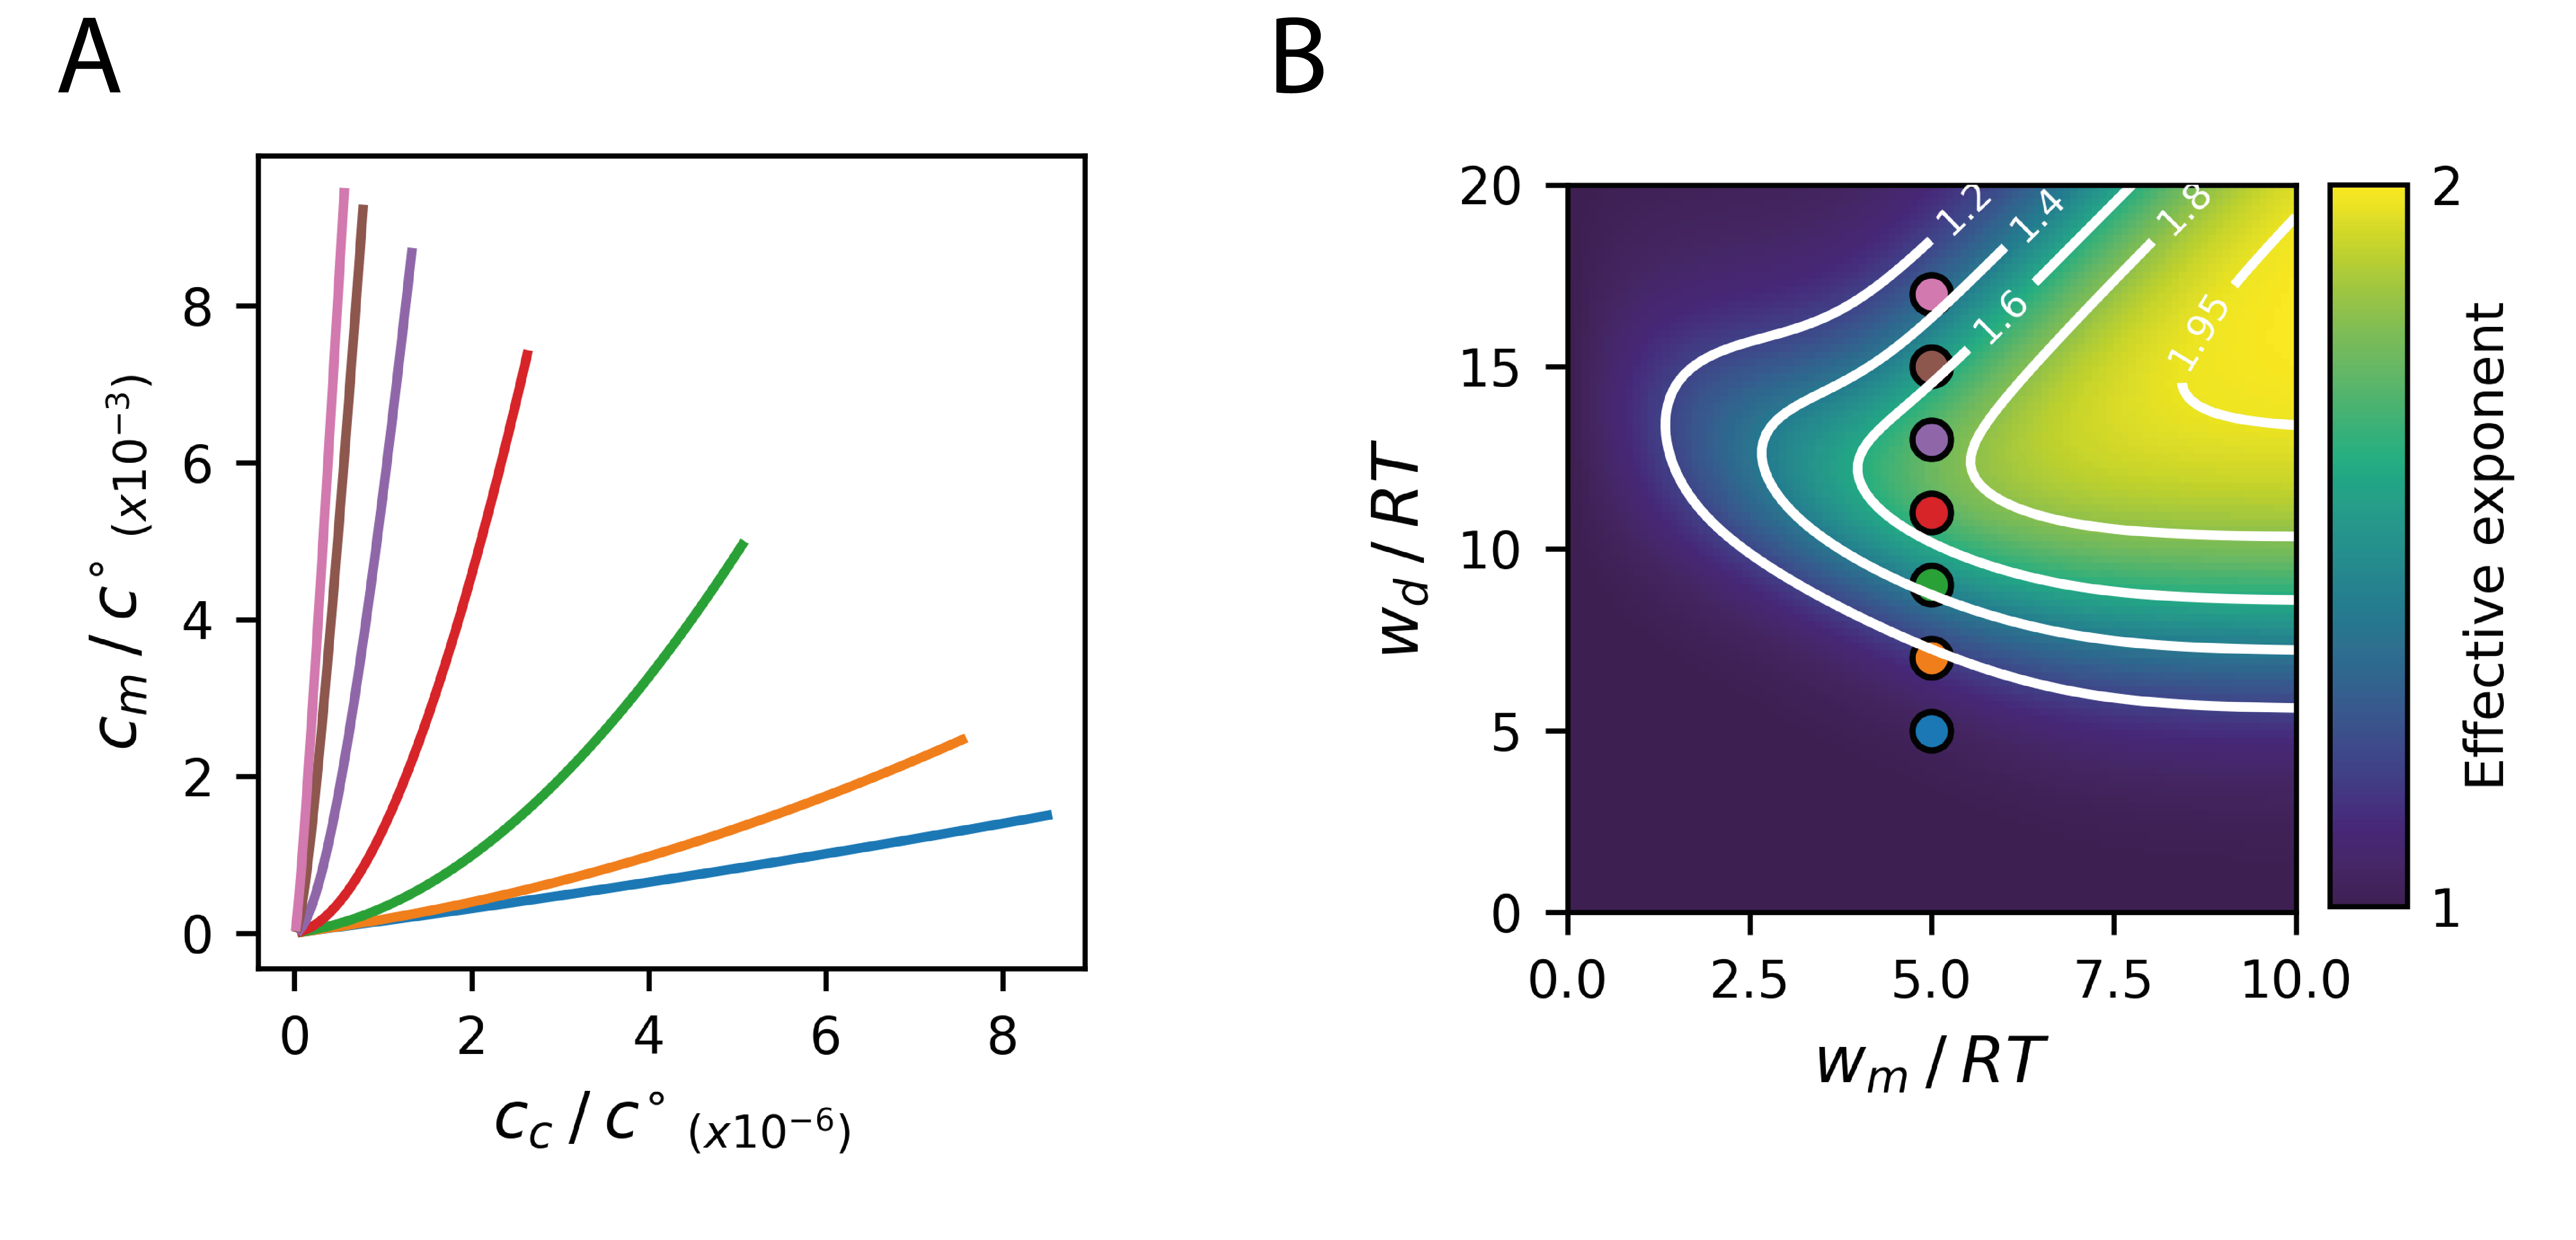
\includegraphics[scale=0.9]{thermodynamic_model_feedback}
\setlength{\abovecaptionskip}{20pt}
\centering
\mycaption{Title}{Caption}
\end{figure}

\subsection{Quantitative analysis of PAR-2 membrane binding kinetics}

\subsection{Discussion}

%%%%%%%%%%%%%%%%%%%%%%%%%%%%%%%%%%%%%%%%%%%%%%%%%%%%%%%%%%
\clearpage
\section{Direct experimental manipulation of dimerisation}

Text

%%%%%%%%%%%%%%%%%%%%%%%%%%%%%%%%%%%%%%%%%%%%%%%%%%%%%%%%%%
\clearpage
\section{Modelling dimerisation-driven positive feedback in the PAR network}

Text

%%%%%%%%%%%%%%%%%%%%%%%%%%%%%%%%%%%%%%%%%%%%%%%%%%%%%%%%%%
\clearpage
\section{Discussion}

Text

%%%%%%%%%%%%%%%%%%%%%%%%%%%%%%%%%%%%%%%%%%%%%%%%%%%%%%%%%%
\clearpage
\section{Materials and methods}

Text

\subsection{Worm maintenance}
\subsection{Generating transgenic lines by CRISPR}
\subsection{Microscopy}
\subsection{Full-length PAR-2 purification}
\subsection{Ubiquitination assays}
\subsection{PAR-2 RING domain fragment purification}
\subsection{SEC-MALS}
\subsection{Image analysis}
\subsection{Modelling methods}

%%%%%%%%%%%%%%%%%%%%%%%%%%%%%%%%%%%%%%%%%%%%%%%%%%%%%%%%%%
\clearpage
\section{Bibliography}

\end{document}
